% 6-10 pages, 9pt font
%
% Topics:
%
% * Machine learning based autotuning.
% * Representative benchmarking.
% * Automatic fault tolerance.
% * Run-time adaption.
%

% The following \documentclass options may be useful:
%
% preprint      Remove this option only once the paper is in final form.
% 10pt          To set in 10-point type instead of 9-point.
% 11pt          To set in 11-point type instead of 9-point.
% authoryear    To obtain author/year citation style instead of numeric.
\documentclass[nonatbib,preprint,9pt]{sigplanconf}

%%%%%%%%%%%%%%%%%%%%%%%%%
%% Document and Layout %%
%%%%%%%%%%%%%%%%%%%%%%%%%

% Fix for multiple "No room for a new \dimen" errors.
%
% See: http://tex.stackexchange.com/questions/38607/no-room-for-a-new-dimen
%
\usepackage{etex}

\usepackage[utf8]{inputenc}

% Fix for "'babel/polyglossia' detected but 'csquotes' missing"
% warning. NOTE: Include after inputenc.
%
\usepackage{csquotes}

% Make internal macro definitions accessible,
% e.g. \@title, \@date \@author.
\makeatletter

% Multi-column support.
\usepackage{multicol}

% A useful package which includes macros like \ifdef{}{}{}:
%
\usepackage{etoolbox}

% Uncomment the following line to remove column separation:
%
%\setlength{\columnsep}{5mm}

% Allow user-defined warning and error filters.
%
\usepackage{silence}


%%%%%%%%%%%%%%%%%%%%%
% Table of Contents %
%%%%%%%%%%%%%%%%%%%%%

% % Set chapter and section numbering depth:
% %
% \setcounter{secnumdepth}{2}


%%%%%%%%%%%%%%%%
% Bibliography %
%%%%%%%%%%%%%%%%
\usepackage[%
    backend=biber,
    style=numeric-comp,
    % style=numeric-comp,  % numerical-compressed
    sorting=none,        % nty,nyt,nyvt,anyt,anyvt,ynt,ydnt,none
    sortcites=true,      % sort \cite{b a d c}: true,false
    block=none,          % space between blocks: none,space,par,nbpar,ragged
    indexing=false,      % indexing options: true,false,cite,bib
    citereset=none,      % don't reset cites
    isbn=false,          % print ISBN?
    url=true,            % print URL?
    doi=false,           % print DOI?
    natbib=true,         % natbib compatability
  ]{biblatex}

% % Filter annoying and unavoidable biblatex warning:
\WarningFilter{biblatex}{Patching footnotes failed}

% Reduce the font size of the bibliography:
% \renewcommand{\bibfont}{\normalfont\scriptsize}

% Determine which BibTeX file to use:
%
% If available, use my Mendeley BibTex library, located in the home
% directory. Note that this is a relative path and will break if
% either this file or the BibTex library are moved. If the library is
% not present, use the local refs.bib file.
\newcommand{\BibResourceGlobal}{../../library.bib}
\newcommand{\BibResourceLocal}{refs.bib}

\IfFileExists{\BibResourceGlobal}
  {\newcommand{\BibResource}{\BibResourceGlobal}}
  {\newcommand{\BibResource}{\BibResourceLocal}}

\addbibresource{\BibResource}


%%%%%%%%%%%%%%
% Appendices %
%%%%%%%%%%%%%%

% Appendix package. Documentation:
%
%  http://mirror.ox.ac.uk/sites/ctan.org/macros/latex/contrib/appendix/appendix.pdf
%
% Package options:
%
% toc      - Put a header (e.g., `Appendices') into the Table of Contents
%            (the ToC) before listing the appendices. (This is done by
%            calling the \addappheadtotoc command.)
% page     - Puts a title (e.g., `Appendices') into the document at the
%            point where the appendices environment is begun. (This is
%            done by calling the \appendixpage command.)
% title    - Adds a name (e.g., `Appendix') before each appendix title in
%            the body of the document. The name is given by the value
%            of \appendixname. Note that this is the default behaviour
%            for classes that have chapters.
% titletoc - Adds a name (e.g., `Appendix') before each appendix listed
%            in the ToC. The name is given by the value
%            of \appendixname.
% header   - Adds a name (e.g., `Appendix') before each appendix in page
%            headers.  The name is given by the value
%            of \appendixname. Note that this is the default behaviour
%            for classes that have chapters.
\usepackage[title, titletoc]{appendix}


%%%%%%%%%%%%%%%%%%%%%%%%%%%%%%%%%%%%%
%% Figures, footnotes and listings %%
%%%%%%%%%%%%%%%%%%%%%%%%%%%%%%%%%%%%%

%\usepackage{float}
%\restylefloat{figure}

% Use bold ``(Figure|Table|Listing)'' caption text.
%\usepackage[margin=1cm]{caption}

% Set the font for captions.
% \renewcommand{\captionfont}{\small}
% Set the font for caption labels.
% \renewcommand{\captionlabelfont}{\footnotesize\bf}

% Use arabic numbers for footnote.
%\renewcommand{\thefootnote}{\arabic{footnote}}

% Ensure that footnotes always appear at the bottom of pages.
%\usepackage[bottom]{footmisc}

% Reset the footnote counter on every page.
%\usepackage{perpage}
%\MakePerPage{footnote}

% Pre-requisites for rendering upquotes in listings package.
\usepackage[T1]{fontenc}
\usepackage{lmodern}
\usepackage{textcomp}

% Pseudo-code listings.
\usepackage{algorithm}
\usepackage{algpseudocode}
\newcommand{\Break}{\State \textbf{break} }
\algblockdefx[Loop]{Loop}{EndLoop}[1][]{\textbf{Loop} #1}{\textbf{End
    Loop}}

\algrenewcommand\ALG@beginalgorithmic{\footnotesize}

% Code listings.
\usepackage{listings}

% Set \ttfamily to use courier fonts.
%
% See: http://tex.stackexchange.com/a/33686
%
\usepackage{courier}

\lstset{frame=bt,                    % Add top and bottom frame lines
        breaklines=true,             % Force line wrapping
        captionpos=b,                % Place caption below listing
        numbers=left,                % Add left-side line numbers
        basicstyle=\scriptsize\ttfamily, % Set font size and type
        showstringspaces=false,      % Don't show visible whitespace
        numberstyle=\tiny,
        upquote=true,                % Use upright quotes, not curly
        commentstyle=\bfseries}      % Embolden comments

% Use (*@ @*) to escape LaTeX commands within listings.
\lstset{escapeinside={(*@}{@*)}}

% Add 10pt space between chapters in TOC listings entries:
%\let\Chapter\chapter
%\def\chapter{\addtocontents{lol}{\protect\addvspace{10pt}}\Chapter}


%%%%%%%%%%%%%%%%%%%%%%%%
%% Graphics and maths %%
%%%%%%%%%%%%%%%%%%%%%%%%
\usepackage{amsmath}

% Vector notation, e.g. \vv{x}:
%
\usepackage{esvect}

% Additional amsmath symbols, see:
%
% http://texblog.org/2007/08/27/number-sets-prime-natural-integer-rational-real-and-complex-in-latex/
%
\usepackage{amsfonts}
\usepackage{amssymb}

\usepackage{graphicx}
\usepackage{mathtools}
\usepackage{tikz}
\usepackage{tikz-qtree}

% Provide bold font face in maths.
\usepackage{bm}

\usepackage{subcaption}
\expandafter\def\csname ver@subfig.sty\endcsname{}

% Define an 'myalignat' command which behave as 'alignat' without the
% vertical top and bottom padding. See:
%     http://www.latex-community.org/forum/viewtopic.php?f=5&t=1890
\newenvironment{myalignat}[1]{%
  \setlength{\abovedisplayskip}{-.7\baselineskip}%
  \setlength{\abovedisplayshortskip}{\abovedisplayskip}%
  \start@align\z@\st@rredtrue#1
}%
{\endalign}

% Define additional operators:
\DeclareMathOperator*{\argmin}{arg\,min}
\DeclareMathOperator*{\argmax}{arg\,max}

\DeclareMathOperator*{\gain}{Gain}

% Skeleton operators.
\DeclareMathOperator*{\map}{Map}
\DeclareMathOperator*{\reduce}{Reduce}
\DeclareMathOperator*{\scan}{Scan}
\DeclareMathOperator*{\stencil}{Stencil}
\DeclareMathOperator*{\zip}{Zip}
\DeclareMathOperator*{\allpairs}{All\,Pairs}

% Maths plots using pgfplots, see:
%
%     http://pgfplots.sourceforge.net/pgfplots.pdf
%
\usepackage{pgfplots}

% Disable compatability mode.
%
\pgfplotsset{compat=1.12}

% Gantt charts using pgfgantt, see:
%
%     http://www.ctan.org/pkg/pgfgantt
%
\usepackage{pgfgantt}

% Fix milestone aspect ratio by defining a custom element.
\newganttchartelement*{mymilestone}{
  mymilestone/.style={
    shape=diamond,
    inner sep=2pt,
    draw=black,
    top color=black,
    bottom color=black,
  }
}

% Tikz flowchart configuration.
\usetikzlibrary{shapes,arrows,shadows,fit,backgrounds}
\tikzstyle{decision} = [diamond,
                        draw,
                        text width=4.5em,
                        text badly centered,
                        node distance=3cm,
                        inner sep=0pt]
\tikzstyle{block}    = [rectangle,
                        draw,
                        text width=5em,
                        text centered,
                        node distance=3cm,
                        minimum height=4em,
                        inner sep=.2cm]
\tikzstyle{line}     = [draw, -latex']

% Add dirtree picture style, see:
%
%     http://tex.stackexchange.com/a/34268
%
\newcount\dirtree@lvl
\newcount\dirtree@plvl
\newcount\dirtree@clvl
\def\dirtree@growth{%
  \ifnum\tikznumberofcurrentchild=1\relax
    \global\advance\dirtree@plvl by 1
    \expandafter\xdef\csname dirtree@p@\the\dirtree@plvl\endcsname{\the\dirtree@lvl}
  \fi
  \global\advance\dirtree@lvl by 1\relax
  \dirtree@clvl=\dirtree@lvl
  \advance\dirtree@clvl by -\csname dirtree@p@\the\dirtree@plvl\endcsname
  \pgf@xa=0.33cm\relax
  \pgf@ya=-\baselineskip\relax
  \pgf@ya=\dirtree@clvl\pgf@ya
  \pgftransformshift{\pgfqpoint{\the\pgf@xa}{\the\pgf@ya}}%
  \ifnum\tikznumberofcurrentchild=\tikznumberofchildren
    \global\advance\dirtree@plvl by -1
  \fi
}
\tikzset{
  dirtree/.style={
    growth function=\dirtree@growth,
    every node/.style={anchor=north},
    every child node/.style={anchor=west},
    edge from parent path={(\tikzparentnode\tikzparentanchor) |- (\tikzchildnode\tikzchildanchor)}
  }
}

% UML sequence diagram macros, see:
%
%     https://code.google.com/p/pgf-umlsd/
%
% Options:
%
%     underline - Underline object names
%
\usepackage[underline=false]{pgf-umlsd}

% Support for SVG graphics.
%
% NOTE that you must pass the "--shell-escape" argument to pdflatex to
% compile. NOTE also that images *MUST* be placed within the graphics
% path.
\usepackage{svg}
\graphicspath{{img/}}

%%%%%%%%%%%%%%%%%%%%%%
%% Tables and lists %%
%%%%%%%%%%%%%%%%%%%%%%

% Required to use labm8 exported tables.
%
\usepackage{booktabs}

% Required for full page-width tables.
\usepackage{tabularx}

%\usepackage{enumitem}
%\setenumerate{itemsep=0pt}

% Use no left margin for lists:
%\setlist{leftmargin=*}

\usepackage{longtable}

% Define column types L, C, R with known text justification and fixed
% widths:
\usepackage{array}
\newcolumntype{L}[1]{>{\raggedright\let\newline\\\arraybackslash\hspace{0pt}}m{#1}}
\newcolumntype{C}[1]{>{\centering\let\newline\\\arraybackslash\hspace{0pt}}m{#1}}
\newcolumntype{R}[1]{>{\raggedleft\let\newline\\\arraybackslash\hspace{0pt}}m{#1}}


%%%%%%%%%%%%%%%%%%%%%%%%%%%%%
%% Typesetting and symbols %%
%%%%%%%%%%%%%%%%%%%%%%%%%%%%%

% Adjustable font sizes in \Verbatim{}
\usepackage{fancyvrb}

%\usepackage{titlesec}
% Set section and paragraph heading fonts:
%\titleformat*{\section}{\Large\bfseries}
%\titleformat*{\subsection}{\normalsize\bfseries}
%\titleformat*{\subsubsection}{\normalsize}
%\titleformat*{\paragraph}{\large\bfseries}
%\titleformat*{\subparagraph}{\large\bfseries}

% Set section heading margins. Usage:
% \titlespacing*{<command>}{<left>}{<before>}{<after>}
%\titlespacing*{\section}{0pt}{.6em}{.3em}
%\titlespacing*{\subsection}{0pt}{.6em}{.2em}

% Set paragraph indentation size. Default is 15pt.
%\setlength{\parindent}{10pt}

% The line spacing can be globally set using \linespread:
%
% \linespread{1.2}

% Add a command \hr{} which will draw a horizontal rule the width of
% the text.
%
\newcommand{\hr}{\noindent\makebox[\linewidth]{\rule{\textwidth}{0.2pt}}}

% Add a command \br{} which will create a horizontal space of exactly
% one line height.
%
\newcommand{\br}{\hspace{\baselineskip}}

% Define a command to allow word breaking.
\newcommand*\wrapletters[1]{\wr@pletters#1\@nil}
\def\wr@pletters#1#2\@nil{#1\allowbreak\if&#2&\else\wr@pletters#2\@nil\fi}

% Define a command to create centred page titles.
\newcommand{\centredtitle}[1]{
  \begin{center}
    \large
    \vspace{0.9cm}
    \textbf{#1}
  \end{center}}

% Support hyperlinks using the \hyperref, \url and \href
% macros. Usage:
%
%    \hyperref[label_name]{''link text''}
%
%    \url{<my_url>}
%
%    \href{<my_url>}{<description>}
%
\usepackage{hyperref}

% Disable colored borders of links, cross-references etc in PDF output
\hypersetup{pdfborder={0 0 0}}

% Provide generic commands \degree, \celsius, \perthousand, \micro
% and \ohm which work both in text and maths mode.
\usepackage{gensymb}

%%%%%%%%%%%%%%%%%%%%%%%%%%%%%%%%%
%% Placeholder text generation %%
%%%%%%%%%%%%%%%%%%%%%%%%%%%%%%%%%

% Use either \blindtext or \libpsum to generate placeholder text. Also
% note the macros \blinditemize, \blindenumerate, \blinddescription.
\usepackage[english]{babel}
\usepackage{blindtext}
\usepackage{lipsum}


\begin{document}

\special{papersize=8.5in,11in}
\setlength{\pdfpageheight}{\paperheight}
\setlength{\pdfpagewidth}{\paperwidth}

\conferenceinfo{HLPGPGPU '16}{Month d--d, 20yy, City, ST, Country}
\copyrightyear{2016}
\copyrightdata{978-1-nnnn-nnnn-n/yy/mm}
\doi{nnnnnnn.nnnnnnn}

% Uncomment one of the following two, if you are not going for the
% traditional copyright transfer agreement.

%\exclusivelicense                % ACM gets exclusive license to publish,
                                  % you retain copyright

%\permissiontopublish             % ACM gets nonexclusive license to publish
                                  % (paid open-access papers,
                                  % short abstracts)

% \titlebanner{banner above paper title}        % These are ignored unless
% \preprintfooter{HLPGPGPU workshop '16}   % 'preprint' option specified.

% \title{Robust Autotuning of Stencil codes for GPUs with OmniTune}
% \title{Towards robust cross-architecture GPGPU patterns autotuning}
\title{Towards Collaborative Performance Tuning of Algorithmic Skeletons}

% \subtitle{Subtitle Text, if any}

\authorinfo{Chris Cummins\and Pavlos Petoumenos \and Michel Steuwer \and Hugh Leather}
           {University of Edinburgh}
           {c.cummins@ed.ac.uk, ppetoume@inf.ed.ac.uk, michel.steuwer@ed.ac.uk, hleather@inf.ed.ac.uk}

\maketitle

\begin{abstract}
  The physical limitations of microprocessor design have forced the
  industry towards increasing heterogeneous designs to extract
  performance. This trend has not been matched with adequate software
  tools, leading to a growing disparity between the availability of
  parallelism and the ability for application developers to exploit
  it.

  Algorithmic skeletons simplify parallel programming by providing
  high-level, reusable patterns of computation. Achieving performant
  skeleton implementations is a difficult task; skeleton authors must
  attempt to anticipate and tune for a wide range of architectures and
  use cases. This results in implementations that target the general
  case and cannot provide the performance advantages that are gained
  from tuning low level optimisation parameters. Autotuning combined
  with machine learning offers promising performance benefits in these
  situations, but the high cost of training and lack of available
  tools limits the practicality of autotuning for real world
  programming.

  To address this, we present OmniTune --- an extensible and
  distributed framework for dynamic autotuning of optimisation
  parameters at runtime. OmniTune uses a client-server model with a
  flexible API to support machine learning enabled
  autotuning. Training data is shared across a network of cooperating
  systems, using a collective approach to performance tuning.

  We demonstrate the practicality of OmniTune in a case study using
  the algorithmic skeleton library SkelCL. By automatically tuning the
  workgroup size of OpenCL Stencil skeleton kernels, we show that that
  static tuning across a range of GPUs and programs can achieve only
  $26\%$ of the optimal performance, while OmniTune achieves $92\%$ of
  this maximum, without introducing a significant runtime overhead.
\end{abstract}

% \category{CR-number}{subcategory}{third-level}

% % general terms are not compulsory anymore,
% % you may leave them out
% % \terms
% % term1, term2

% \keywords
% keyword1, keyword2

\section{Introduction}\label{sec:introduction}

General purpose programming with GPUs has been shown to provide huge
parallel throughput, but poses a significant programming challenge,
requiring application developers to master an unfamiliar programming
model (such as provided by CUDA or OpenCL) and architecture (SIMD with
a multi-level memory hierarchy). As a result, GPGPU programming is
often considered beyond the realm of everyday development. If steps
are not taken to increase the accessibility of such parallelism, the
gap between potential and utilised performance will continue to widen
as hardware core counts increases.

Algorithmic skeletons offer a solution to this this
\emph{programmability challenge} by raising the level of
abstraction. This simplifies parallel programming, allowing developers
to focus on solving problems rather than coordinating parallel
resources. Skeletons provide robust parallel implementations of common
patterns of computation which developers parameterise with their
application-specific code~\cite{Gonzalez2010}. This greatly reduces
the challenge of parallel programming, allowing users to structure
their problem-solving logic sequentially, while offloading the
cognitive cost of parallel coordination to the skeleton library
author. The rising number of skeleton frameworks supporting graphics
hardware illustrates the demand for high level abstractions for GPGPU
programming~\cite{Enmyren2010, Marques2013, Nugteren2014a}.


\subsection{The Performance Portability Challenge}

The performance of parallel programs is sensitive to low level
parameter values, and when selecting values for maximising
performance, one size does not fit all. The suitability of parameter
values depends on the program implementation, the target hardware, and
the dataset that is operated upon. Iterative compilation and
autotuning have been shown to help in these cases by automating the
process of tuning parameter values to match individual execution
environments. However, there have been few attempts to develop general
mechanisms for these techniques, and the time taken to develop ad-hoc
autotuning solutions and gather performance data is often
prohibitively expensive.

We believe that by embedding autotuning at the skeletal level, it is
possible to achieve performance with algorithmic skeletons that is
competitive with --- and in some cases, exceeds --- that of hand tuned
parallel implementations which traditionally came at the cost of many
man hours of work from expert programmers to develop.

Incorporating autotuning into algorithmic skeleton libraries has two
key benefits: first, it minimises development effort by requiring only
a modification to the skeleton implementation rather than to every
user program; and second, by targeting a library, it enables a broader
and more substantive range of performance data to be gathered than
with ad-hoc tuning of individual programs.


\subsection{Contributions}

The first key contribution of this work is the design and
implementation of a generic toolset for autotuning: \emph{OmniTune} is
a novel and extensible framework for collaborative autotuning of
optimisation parameters across the life cycle of programs. The second
contribution is the integration of OmniTune with an established
skeleton library for CPU and multi-GPU parallelism,
SkelCL~\cite{Steuwer2011}. We demonstrate that predicting the
workgroup sizes of stencil skeletons across a range of devices and
programs using OmniTune achieves 92\% of the best possible
performance, providing a median speedup of $5.65\times$ over the best
possible statically chosen workgroup size.


\section{Motivation}

\begin{figure}
\centering
\begin{subfigure}[h]{.45\columnwidth}
\centering
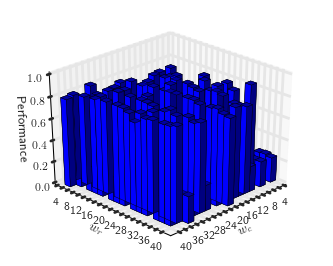
\includegraphics[width=1.0\columnwidth]{img/motivation_1}
\vspace{-1.5em} % Shrink vertical padding
\caption{}
\label{fig:motivation-1}
\end{subfigure}
~%
\begin{subfigure}[h]{.45\columnwidth}
\centering
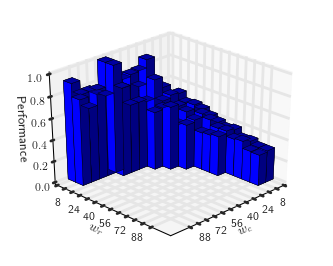
\includegraphics[width=1.0\columnwidth]{img/motivation_2}
\vspace{-1.5em} % Shrink vertical padding
\caption{}
\label{fig:motivation-2}
\end{subfigure}
\caption{%
  The performance of different workgroup sizes for the same stencil
  program on two different devices: (\subref{fig:motivation-1}) Intel
  CPU, (\subref{fig:motivation-2}) NVIDIA GPU.%
}
\label{fig:motivation-arch}
\end{figure}

\begin{figure}
\centering
\begin{subfigure}[h]{.45\columnwidth}
\centering
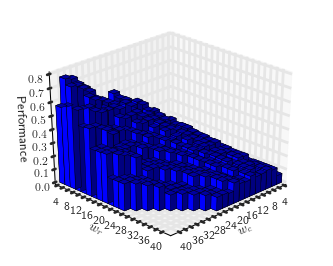
\includegraphics[width=1.0\columnwidth]{img/motivation_3}
\vspace{-1.5em} % Shrink vertical padding
\caption{}
\label{fig:motivation-3}
\end{subfigure}
~%
\begin{subfigure}[h]{.45\columnwidth}
\centering
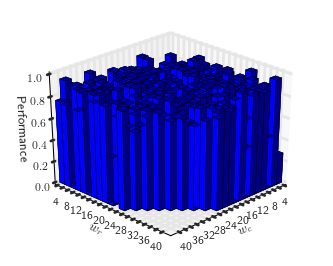
\includegraphics[width=1.0\columnwidth]{img/motivation_4}
\vspace{-1.5em} % Shrink vertical padding
\caption{}
\label{fig:motivation-4}
\end{subfigure}
\caption{%
  The performance of different workgroup sizes for two different
  stencil programs on the same execution device.%
}
\label{fig:motivation-prog}
\end{figure}


In this section we will briefly examine the performance impact of
selecting workgroup size for the SkelCL Stencil skeleton. In OpenCL,
multiple threads are grouped into \emph{workgroups}. The shape and
size of these groups is known to have a big impact on performance. A
full explanation of SkelCL and the workgroup size parameter space is
given Section~\ref{sec:omnitune-skelcl}.

For the SkelCL stencil skeleton, the selection of workgroup size
presents a two dimensional parameter space, consisting of a number of
rows and columns ($w_r \times w_c$).  Plotting the runtime of stencil
programs using different workgroup sizes allows us to compare
performance. Figure~\ref{fig:motivation-arch} shows this performance
comparison for a single stencil program on two different devices,
demonstrating that a good choice of workgroup size is device
dependent. The optimisation space of the same stencil benchmark on
different devices being radically different --- not only does the
optimal workgroup size change between devices, but the performance of
suboptimal workgroup sizes is also dissimilar. The optimisation space
of~\ref{fig:motivation-1} has a grid-like structure, with clear
performance advantages of workgroup sizes at multiples of 8 for
$w_c$. A developer specifically targeting this device would learn to
select workgroup sizes following this pattern. This domain specific
knowledge clearly does not transfer to the device shown
in~\ref{fig:motivation-2}.

In Figure~~\ref{fig:motivation-prog}, we compare the performance of
two different stencil programs on the \emph{same} device, showing that
workgroup size choice is also program dependent. In each of these four
examples, the optimal workgroup size changes, as does the relative
performance of suboptimal parameters. The average speedup of the best
over the worst workgroup size is $37.0\times$, and the \emph{best}
average performance that can be achieved using a single fixed
workgroup size is 63\%.

SkelCL uses a fixed workgroup size. Since both the execution device
and the user-provided stencil code are not known until runtime,
selection of workgroup size should be made dynamically. To the best of
our knowledge, there are no existing systems for runtime autotuning of
arbitrary parameter values, and autotuners are generally developed
ad-hoc and on a per-case basis.


\section{The OmniTune Framework}\label{sec:autotune}

OmniTune is a novel framework for extensible, distributed autotuning
of parameter values at runtime using machine learning. It serves as a
generic platform for developing autotuning solutions, aiming to reduce
the developer and amount of duplicate effort required by ad-hoc
solutions.

and emphasises collaborative, online learning of optimisation
spaces. A client-server architecture with clearly delineated
separation of concerns minimises the code footprint in client
applications, enabling quick re-purposing for autotuning
targets. OmniTune provides a lightweight interface for communication
between each of the components, and aims to strike a balance between
offering a fully featured environment for quickly implementing
autotuning, while providing enough flexibility to cater to a wide
range of use cases. First, we describe the overall structure of
OmniTune and the rationale for the design, followed by the interfaces
and steps necessary to apply OmniTune.


\subsection{System Architecture}

\begin{figure}
\centering
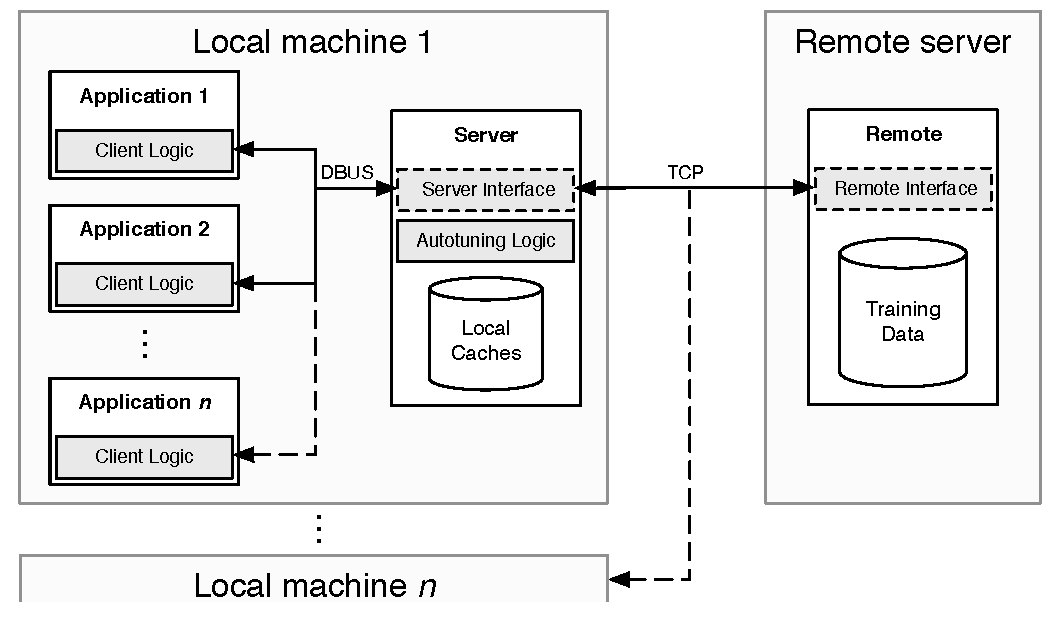
\includegraphics[width=.98\columnwidth]{img/omnitune-system-overview.pdf}
\caption[OmniTune system diagram]{%
  OmniTune system architecture, showing the separate components and
  the one to many relationship between servers to client applications,
  and remotes to servers.%
}
\label{fig:omnitune-system-overview}
\end{figure}

Common implementations of autotuning in the literature either embed
the autotuning logic within the each target application, or take a
standalone approach in which the autotuner is a program which must be
invoked by the user to tune a target application. Embedding the
autotuner within each target application has the advantage of
providing ``always-on'' behaviour, but is infeasible for complex
systems in which the cost of building machine learning models must be
added to each program run. The standalone approach separates the
autotuning logic, at the expense of adding one additional step to the
build process. The approach taken in OmniTune aims to combine the
advantages of both techniques by implementing autotuning \emph{as a
  service}, in which a standalone autotuning server provides the heavy
lifting of training data and machine learning model management, with a
minimal set of lightweight communication logic to be embedded in
target applications.

OmniTune is built around a three tier client-server model, shown in
Figure~\ref{fig:omnitune-system-overview}. The applications which are
to be autotuned are the \emph{clients}. These clients communicate with
a system-wide \emph{server}, which handles autotuning requests. The
server communicates and caches data sourced from a \emph{remote}
server, which maintains a global store of all autotuning data.

There is a many to one relationship between clients, servers, and
remotes, such that a single remote may handle connections to multiple
servers, which in turn may accept connections from multiple
clients. This design has two primary advantages: the first is that it
decouples the autotuning logic from that of the client program,
allowing developers to easily repurpose the autotuning framework to
target additional optimisation parameters without a significant
development overhead for the target applications; the second advantage
is that this enables collective tuning, in which training data
gathered from a range of devices can be accessed and added to by any
OmniTune server.

The OmniTune framework is implemented as a set of Python classes,
which are inherited from or implemented to target specific autotuning
cases. The generic implementation of OmniTune's server and remote
components consists of 8987 lines of Python and MySQL code. No client
logic is provided, since that is use case dependent (See
Section~\ref{sec:omnitune-skelcl} for an example implementation for
SkelCL). Inter-process communication between client programs and the
server uses the D-Bus protocol. D-Bus is cross-platform, and bindings
are available for most major programming languages, allowing
flexibility for use with a range of clients. Communication between
servers and remotes uses TCP/IP (we used an Amazon Web Services
database instance for development).


\subsection{Interfaces}

Key design elements of OmniTune are the interfaces exposed by the
server and remote components.

\paragraph{Client-Server Interface} An OmniTune server exposes a
public interface over D-Bus with four operations. Client applications
invoke these methods to request parameter values, submit new training
observations, and refuse suggested parameters:
%
\begin{itemize}
\item \textsc{Request}$(x) \to p$\\*Given explanatory variables $x$,
  request the parameter values $p$ which are expected to provide
  maximum performance.
\item \textsc{RequestTraining}$(x) \to p$\\*Given explanatory
  variables $x$, allow the server to select parameter values $p$ for
  evaluating their fitness.
\item \textsc{Submit}$(x, p, y)$\\*Submit an observed measurement of
  fitness $y$ for parameter values $p$, given explanatory variables
  $x$.
\item \textsc{Refuse}$(x, p)$\\*Refuse parameter values $p$, given a
  set of explanatory variables $x$. Once refused, those parameters are
  blacklisted and will not be returned by any subsequent calls to
  \textsc{Request()} or \textsc{RequestTraining()} for the same
  explanatory variables $x$.
\end{itemize}
%
% This set of operations enables the core functionality of an autotuner,
% while providing flexibility for the client to control how and when
% training data is collected.

\paragraph{Server-Remote Interface} The role of the remote is to
provide bookkeeping of training data for machine learning. Remotes
allow shared access to data from multiple servers using a
transactional communication pattern, supported by two methods:
%
\begin{itemize}
\item \textsc{Push}$(\bf{x}, \bf{p}, \bf{y})$\\*Asynchronously submit
  training data as three lists: explanatory variables $\bf{x}$,
  parameter values $\bf{p}$, and observed outcomes $\bf{y}$.
\item \textsc{Pull}$() \to (\bf{x}, \bf{p}, \bf{y})$\\*Request
  training data as three lists: explanatory variables $\bf{x}$,
  parameter values $\bf{p}$, and observed outcomes $\bf{y}$.
\end{itemize}
%
Figure~\ref{fig:omnitune-comms} shows an example communication pattern
between the three components of an OmniTune system using these
interfaces. In the example, a server first requests training data from
the remote. A client application then performs a training phase in
which it requests a set of parameters for training, evaluates the
performance of the parameters, and then submits a measured value,
which the server uses to update the remote. After training, another
client program requests a set of parameters for performance, refuses
them, and makes a new request.

\begin{figure}
\centering
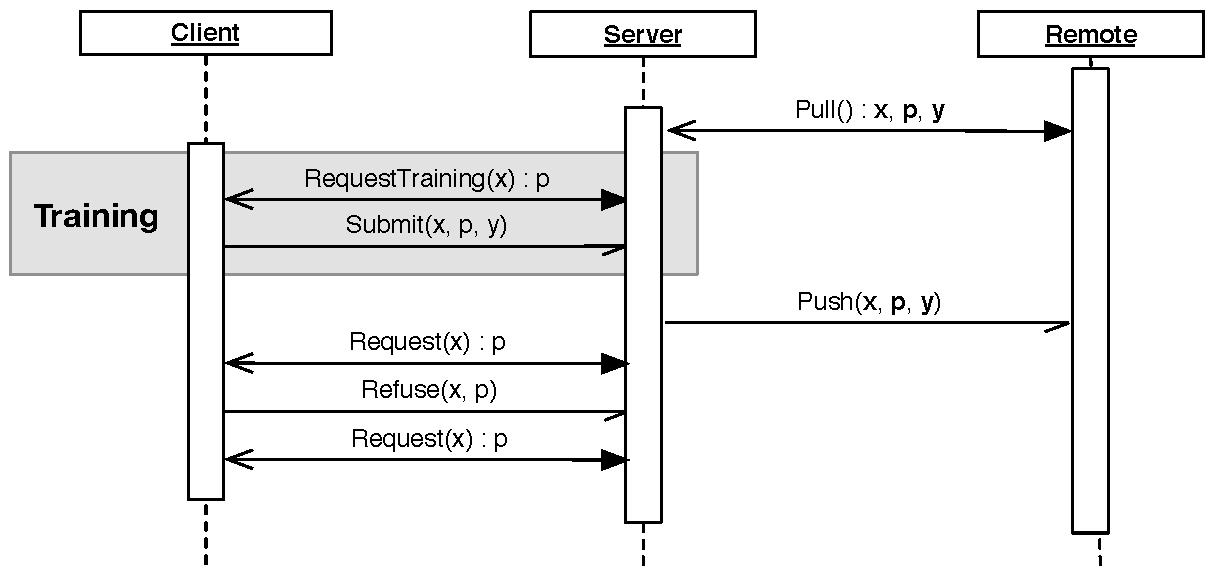
\includegraphics[width=1.0\columnwidth]{img/omnitune-comms}
\caption{%
  An example communication pattern between OmniTune components,
  showing an offline training phase.%
}
\label{fig:omnitune-comms}
\end{figure}


\subsection{Autotuning Behaviour}

OmniTune supports autotuning using a separate offline training phase,
online training, or a mixture of both. For each autotuning-capable
machine, the server acts as an intermediary between training data and
by hosting the machine learning logic. On launch, a server requests
the latest training data from the remote, which it uses to build the
relevant models for performing prediction of optimisation parameter
values. If additional training data is gathered by the server, this
can be uploaded to the remote.

The autotuning technique is application-specific, and can depend on
the type of parameter being tuned (e.g. a binary flag or one or more
numeric values). The server contains a library of machine learning
tools to perform parameter prediction, interfacing with the popular
datamining software suite
Weka\footnote{\url{http://www.cs.waikato.ac.nz/ml/weka/}} using a Java
Native Interface. The provided tools include classifiers, regressors,
and a selection of meta-learning algorithms.

OmniTune servers may perform additional feature extraction of
explanatory variables supplied by incoming client requests. The reason
for performing feature extraction on the server as opposed to on the
client side is that this allows the results of expensive operations
(for example, analysing source code of target applications) to be
cached for use across the lifespan of client applications. The
contents of these local caches are periodically and asynchronously
synced with the remote to maintain a global store of lookup tables for
expensive operations.



\subsection{Usage}

\begin{figure}
\centering
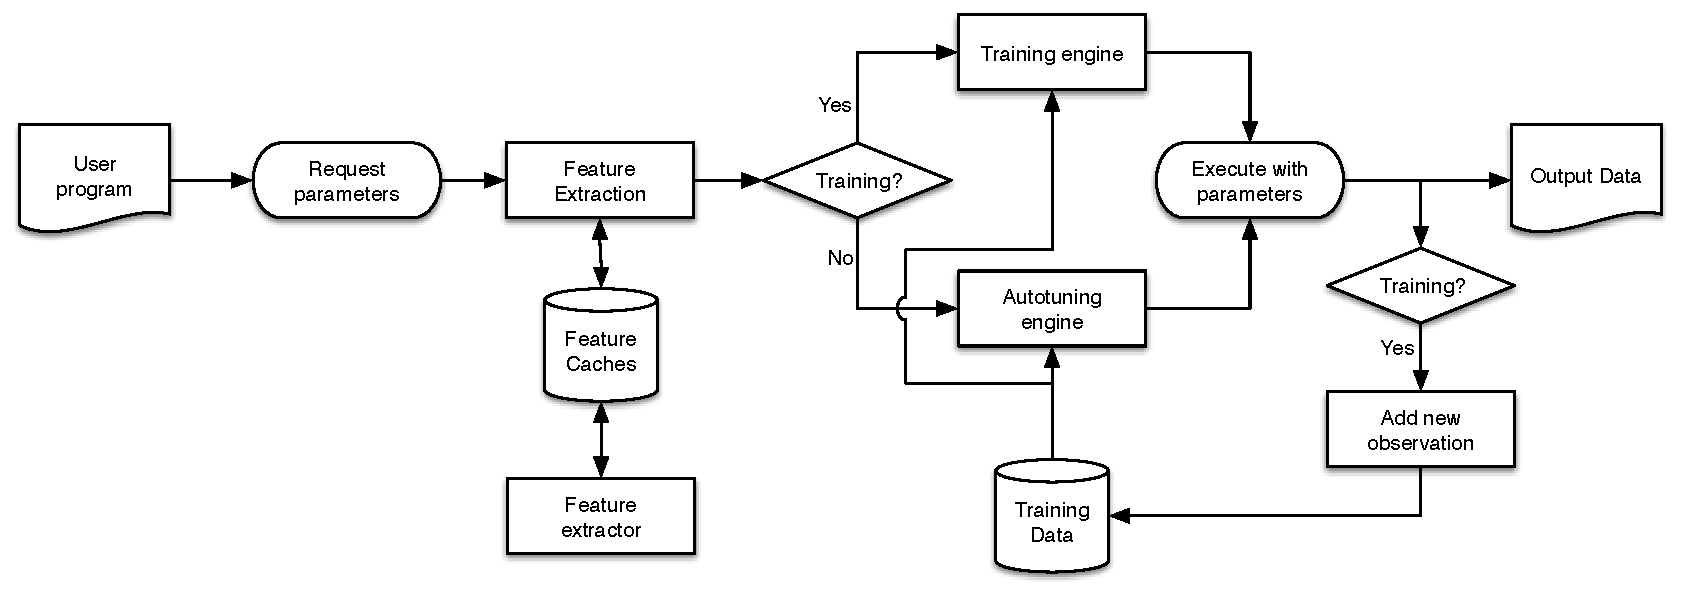
\includegraphics[width=\columnwidth]{img/omnitune-system-flow.pdf}
\caption[Optimisation parameter selection with OmniTune]{%
  Predicting parameter values and collecting training data with
  OmniTune.%
}
\label{fig:omnitune-system-flow}
\end{figure}

To use OmniTune, a developer extends the server class to implement
response handlers for the four public interface operations, and then
insert client code into the target application to call these
operations. The implementation of these response handlers and invoking
client code dictates the type of autotuning methods
supported. Figure~\ref{fig:omnitune-system-flow} shows the flow
diagram for an example OmniTune implementation. TODO: explain! In the
next Section, we will detail the steps required to apply OmniTune to
SkelCL.


\section{Integration of OmniTune with SkelCL}\label{sec:omnitune-skelcl}

In this section we demonstrate the practicality of OmniTune by
integrating the framework with SkelCL. Introduced
in~\cite{Steuwer2011}, SkelCL addresses the parallel programmability
challenge by allowing users to easily harness the power of GPUs and
CPUs for data parallel computing, offering a set of OpenCL
implementations of data parallel skeletons in an object oriented C++
library.

The goal of SkelCL is to enable the transition towards higher-level
programming of GPUs, without requiring users to be intimately
knowledgeable of the concepts unique to OpenCL programming, such as
the memory or execution model. SkelCL has been shown to reduce
programming effort for developing real applications through the use of
robust pattern implementations and automated memory
management. Skeletons are parameterised with user functions which are
compiled into OpenCL kernels for execution on device hardware. SkelCL
supports operations on one or two dimensional arrays of data, with the
Vector and Matrix container types transparently handling lazy
transfers between host and device memory, and supporting partitioning
for multi-GPU execution. SkelCL is freely available and distributed
under dual GPL and academic
licenses\footnote{\url{http://skelcl.uni-muenster.de}}.

\subsection{The Stencil Skeleton}

Stencils are patterns of computation which operate on uniform grids of
data, where the value of each cell is updated based on its current
value and the value of one or more neighbouring elements, called the
\emph{border region}. Figure~\ref{fig:stencil-img} shows the use of a
stencil to apply a Gaussian blur to an image. SkelCL provides a 2D
stencil skeleton which allows users to provide a function which
updates a cell's value, while SkelCL orchestrates the parallel
execution of this function across all cells~\cite{Steuwer2014a}.

The border region is described by a \emph{stencil shape}, which
defines an $i \times j$ rectangular region around each cell which is
used to update the cell value. Stencil shapes may be asymmetrical, and
are defined in terms of the number of cells in the border region to
the north, east, south, and west of each cell. Given a function $f$, a
stencil shape $S$, and an $n \times m$ matrix:
%
\begin{equation}
\scriptsize
% \begin{split}
\stencil \left( f, S,
\begin{bmatrix}
  x_{11} & \cdots & x_{1m} \\
  \vdots & \ddots & \vdots \\
  x_{n1} & \cdots & x_{nm}
\end{bmatrix} \right)
\to
\begin{bmatrix}
  z_{11} & \cdots & z_{1m} \\
  \vdots & \ddots & \vdots \\
  z_{n1} & \cdots & z_{nm}
\end{bmatrix}
% \end{split}
\end{equation}
%
where:
%
\begin{equation}
\scriptsize
z_{ij} = f \left(
\begin{bmatrix}
  x_{i-S_n,j-S_w} & \cdots & x_{i-S_n,j+S_e} \\
  \vdots & \ddots & \vdots \\
  x_{i+S_s,j-S_w} & \cdots & x_{i+S_s,j+S_e}
\end{bmatrix} \right)
\end{equation}
%
For border region elements outside the bounds of the matrix, values
are substituted from either a predefined padding value, or the value
of the nearest element within the matrix, depending on user
preference.

A popular usage of Stencil codes is for iterative problem solving,
whereby a stencil operation is repeated over a range of discrete time
steps $0 \le t \le t_{max}$, and $t \in \mathbb{Z}$. An iterative
stencil operation $g$ accepts a customising function $f$, a Stencil
shape $S$, and a matrix $M$ with initial values $M_{init}$. The value
of an iterative stencil can be defined recursively as:
%
\begin{equation}
\scriptsize
g(f, S, M, t) =
\begin{cases}
  \stencil \left( f, S, g(f, S, M, t-1) \right),& \text{if } t \geq 1\\
  M_{init}, & \text{otherwise}
\end{cases}
\end{equation}
%
Examples of iterative stencils include cellular automata and partial
differential equation solvers. % Another extension of the stencil
% operation accepts an ordered list of customising functions which are
% applied sequentially for each iteration. This has applications for
% multi-stage stencil operations such as Canny Edge Detection, in
% which four distinct stencil operations are performed as a sequence.

In the implementation of the SkelCL stencil skeleton, each element in
the matrix is mapped to a unique thread (known as a \emph{work item}
in OpenCL) which applies the user-specified function. The work items
are then divided into \emph{workgroups} for execution on the target
hardware. Each work-item reads the value of its corresponding matrix
element and the surrounding elements defined by the border
region. Since the border regions of neighbouring elements overlap, the
value of all elements within a workgroup are copied into a
\emph{tile}, allocated as a contiguous region of the fast, but small
local memory. As local memory access times are much faster than that
of global device memory, this greatly reduces the latency of the
border region reads performed by each work item. Changing the size of
workgroups thus affects the amount of local memory required for each
workgroup, and in turn affects the number of workgroups which may be
simultaneously active on the device. While the user defines the data
size and type, the shape of the border region, and the function being
applied to each element, it is the responsibility of the SkelCL
stencil implementation to select an appropriate workgroup size to use.

\begin{figure}
\centering
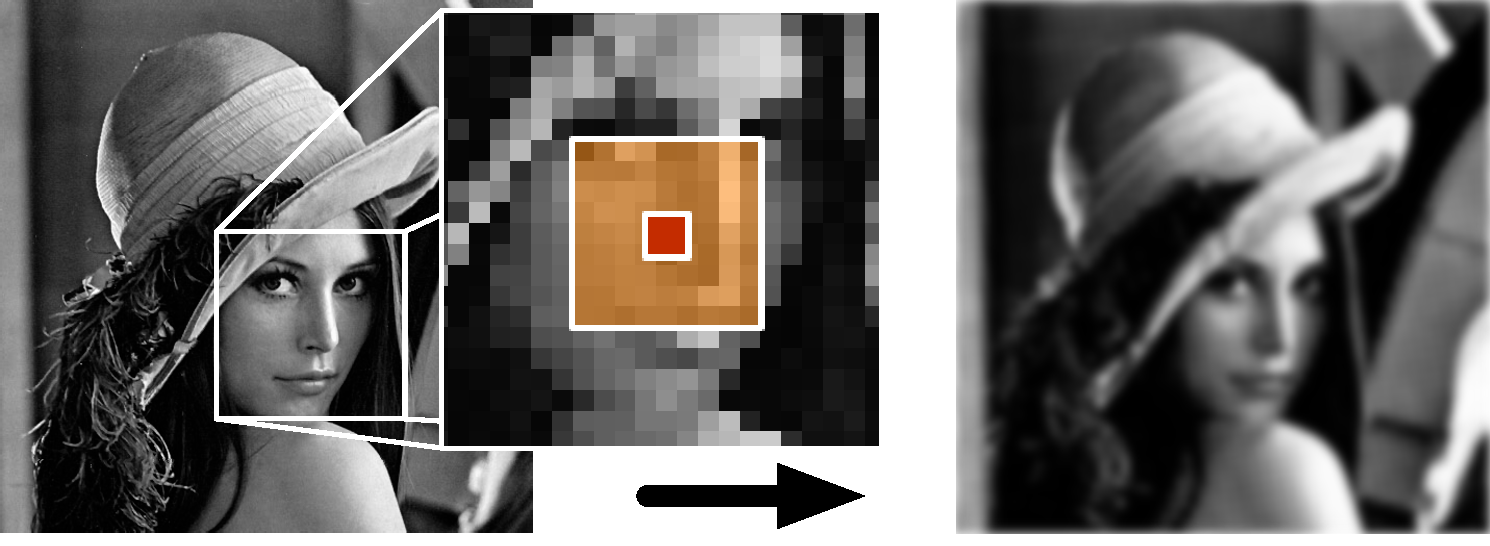
\includegraphics[width=.98\columnwidth]{img/lena-stencil.pdf}
\caption{%
  Application of a Gaussian blur stencil operation to an image, with a
  border region of radius 1. In a Gaussian blur, pixel values are
  interpolated with neighbouring pixels, producing a smoothed effect.%
}
\label{fig:stencil-img}
\end{figure}


\subsection{Optimisation Space}\label{subsec:op-params}

SkelCL stencil kernels are parameterised by a workgroup size $w$,
which consists of two integer values to denote the number of rows and
columns of work items. The space of optimisation parameter values is
subject to hard constraints, and these constraints cannot conveniently
be statically determined. Contributing factors are architectural
limitations, kernel constraints, and refused parameters.  Each OpenCL
device imposes a maximum workgroup size which can be statically
checked by querying the \texttt{clGetDeviceInfo()} API for that
device. These are defined by archiectural limitations of how code is
mapped to the underlying execution hardware. Typical values are powers
of two, e.g.\ 1024, 4096, 8192. At runtime, once an OpenCL program has
been compiled to a kernel, users can query the maximum workgroup size
supported by that particular kernel using the
\texttt{clGetKernelInfo()} API. This value cannot easily be obtained
statically as there is no mechanism to determine the maximum workgroup
size for a given source code and device without first compiling it,
which in OpenCL does not occur until runtime.

Factors which affect a kernel's maximum workgroup size include the
number registers required for a kernel, and the available number of
SIMD execution units for each type of instructions in a kernel. In
addition to satisfying the constraints of the device and kernel, not
all points in the workgroup size optimisation space are guaranteed to
provide working programs. A \emph{refused parameter} is a workgroup
size which satisfies the kernel and architectural constraints, yet
causes a \texttt{CL\_OUT\_OF\_RESOURCES} error to be thrown when the
kernel is enqueued. Note that in many OpenCL implementations, this
error type acts as a generic placeholder and may not necessarily
indicate that the underlying cause of the error was due to finite
resources constraints. We define a \emph{legal} workgroup size as one
which, for a given \emph{scenario} (a combination of program, device,
and dataset), satisfies the architectural and kernel constraints, and
is not refused. The subset of all possible workgroup sizes
$W_{legal}(s) \subset W$ that are legal for a given sceanario $s$ is
then:
%
\begin{equation}
  W_{legal}(s) = \left\{w | w \in W, w < W_{\max}(s) \right\} - W_{refused}(s)
\end{equation}
%
Where $W_{\max}(s)$ can be determined at runtime prior to the kernels
execution, but the set $W_{refused}(s)$ can only be determined
experimentally.

% \subsubsection{Assessing Relative Performance}

%, where an observation is a scenario,
% workgroup size tuple $(s,w)$; a function $t(s,w)$ which returns the
% arithmetic mean of the runtimes for a set of observations; we can
% calculate the speedup $r(s, w_1, w_2)$ of competing workgroup sizes
% $w_1$ over $w_2$ using:
% %
% \begin{equation}
%   r(s, w_1, w_2) = \frac{t(s,w_2)}{t(s,w_1)}\\
% \end{equation}
% %

% \paragraph{Oracle Workgroup Size}

The \emph{oracle} workgroup size $\Omega(s) \in W_{legal}(s)$ of a
scenario $s$ is the $w$ value which provides the lowest mean
runtime. The relative performance $p(s,w)$ of a particular workgroup
against the maximum available performance for that scenario, within
the range $0 \le p(s,w) \le 1$, is the ratio of the runtime of a
program with workgroup size $w$ over the oracle workgroup size
$\Omega(s)$. For a given workgroup size, the average performance
$\bar{p}(w)$ across a set of scenarios $S$ can be found using the
geometric mean of performance relative to the oracle:
%
\begin{equation}
  \bar{p}(w) =
  \left(
    \prod_{s \in S} p(s, w)
  \right)^{1/|S|}
\end{equation}
%
The \emph{baseline} workgroup size $\bar{w}$ is the value which
provides the best average case performance across a set of
scenarios. Such a baseline value represents the \emph{best} possible
performance which can be achieved using a single, statically chosen
workgroup size. By defining $W_{safe} \in W$ as the intersection of
legal workgroup sizes, the baseline can be found using:
%
\begin{align}
W_{safe} &= \cap \left\{ W_{legal}(s) | s \in S \right\}\\
\bar{w} &= \argmax_{w \in W_{safe}} \bar{p}(w)
\end{align}


\subsection{Autotuning Methodology}

The optimisation space presented by the workgroup size of OpenCL
kernels is large, complex, and non-linear. Successfully applying
machine learning to such a space requires plentiful training data, the
careful selection of features, and appropriate machine learning
methods. For the purpose of this work we use a \emph{classification}
approach, in which machine learning is used to correlate patterns
between explanatory variables (features) and the workgroup sizes which
provide optimal performance.

Explanatory variables capture information about the device, program,
and dataset. Device features encode the device type (e.g. CPU or GPU,
integrated or external, connection bus), properties about the host
(e.g.\ system memory, maximum clock frequency), and numerous
properties about the execution device (e.g.\ number of compute units,
local memory size, global caches). Program features include
per-instruction type densities, the total number of basic blocks, and
the total instruction count. They are extracted using static
instruction count passes over an LLVM IR compiled version of the user
stencil implementation. Compilation to bitcode is a relatively
expensive task, so lookup tables are used to cache repeated uses of
the same stencil codes, identified by the source code
checksum. Dataset features include the data type and dimensions of the
SkelCL container type.

% \paragraph{Training}

To collect training data, we run multiple iterations of a stencil
operation to enumerate the workgroup size optimisation space, and use
the OpenCL's Profiling API to record stencil kernel execution times in
the client application, which are then submitted to the OmniTune
server. The \textsc{RequestTraining}$(x)$ server interface returns a
workgroup size with a randomly selected even number of rows and
columns up to the maximum allowed:
$\left\{ 2x \in \mathbb{Z} | 1 \le x < \frac{W_{max}(s)}{2} \right\}$.

A parameterised template substitution engine is used to generate
synthetic stencil applications for gathering performance
data. Stencils templates are parameterised with a border region size
and \emph{complexity}, a simple metric which broadly dictates the
number of operations in a given stencil code.

% \paragraph{Prediction}

Using the OmniTune framework, the challenge is to design a system
which, given a set of prior observations of the empirical performance
of stencil codes with different workgroup sizes, predict workgroup
sizes for \emph{unseen} stencils which will maximise the
performance. Once the performance of different workgroup sizes for a
particular scenario are gathered, the set of features describing the
scenario is labelled with the oracle workgroup size, which is used as
the target class to train a classifier.

This approach presents the problem that after training, there is no
guarantee that the set of workgroup sizes which may be predicted is
within the set of legal workgroup sizes for future scenarios:
%
\begin{equation}
  \bigcup_{\forall s \in S_{testing}} W_{legal}(s) \nsubseteq W_{training}
\end{equation}
%
This may result in a classifier predicting a workgroup size which is
not legal for a scenario, $w \not\in W_{legal}(s)$, either because it
exceeds $W_{\max}(s)$, or because the parameter is refused. For these
cases, a \emph{nearest neighbour} approach is used to select the
workgroup size which is expected to be legal and has the lowest
Euclidian distance to the prediction.

\paragraph{Implementation}

of which 976 is dedicated to the SkelCL frontend. By design, the
client-server model minimises the impact of number of modifications
that are required to enable autotuning in client applications. The
only modification required is to replace the hardcoded values for
workgroup size with a subroutine to request a workgroup size from the
OmniTune server over a D-Bus connection.

For classification, four classifiers are supported, chosen for their
contrasting properties: Naive Bayes, SMO, J48 Decision tree, and
Random Forest.


\section{Experimental Setup}

This section describes an exhaustive enumeration of the workgroup size
optimisation space for 429 combinations of architecture, program, and
dataset. It contains the methodology used to collect empirical
performance data on which to base performance comparisons of different
workgroup sizes, and the steps necessary to obtain repeatable results.

A full enumeration of the workgroup size optimisation spaces was
performed across synthetically generated benchmarks and four reference
stencil benchmarks: Canny Edge Detection, Conway's Game of Life, Heat
Equation, and Gaussian Blur. Performance data was collected from 7
experimental platforms, comprising 4 GPU devices: AMD Tahiti 7970,
Nvidia GTX 590, Nvidia GTX 690, Nvidia GTX TITAN; and 3 CPU devices:
Intel i5-2430M, Intel i5-4570, i7-3820.  Each platform was unloaded,
frequency governors disabled, and benchmark processes set to the
highest priority available to the task scheduler. Datasets and
programs were stored in an in-memory file system. For each combination
of scenario and workgroup size, a minimum of 30 samples were
recorded. Dataset sizes of size $512\times512$, $1024\times1024$,
$2048\times2048$, and $4096\times4096$ were used.

Program behavior is validated by comparing program output against a
gold standard output collected by executing each of the real-world
benchmarks programs using the baseline workgroup size. The output of
real-world benchmarks with other workgroup sizes is compared to this
gold standard output to test for correct program execution.

Five different classification algorithms are used to predict oracle
workgroup sizes, chosen for their contrasting properties: Naive Bayes,
SMO, Logistic Regression, J48 Decision tree, and Random
Forest~\cite{Han2011}. For regression, a Random Forest with regression
trees is used, chosen because of its efficient handling of large
feature sets compared to linear models~\cite{Breiman1999}. The
autotuning system is implemented in Python as a system daemon. SkelCL
stencil programs request workgroup sizes from this daemon, which
performs feature extraction and classification.


\section{Evaluation}\label{sec:evaluation}

This section evaluates the performance of OmniTune when tasked with
selecting workgroup sizes for SkelCL stencil codes. First I discuss
measurement noise present in the experimental results, and the methods
used to accommodate for it. Then I examine the observed effect that
workgroup size has on the performance of SkelCL stencils. The
prediction quality of OmniTune is scrutinised for portability across
programs, devices, and datasets.

% The effectiveness of each of the autotuning techniques described in
% the previous sections is evaluated using multiple different machine
% learning algorithms.

% % \paragraph{Overview of Experimental Results}

The experimental results consist of measured runtimes for a set of
\emph{test cases}, collected using the methodology explained in the
previous section. Each test case $\tau_i$ consists of a scenario,
workgroup size pair $\tau_i = (s_i,w_i)$, and is associated with a
\emph{sample} of observed runtimes from multiple runs of the
program. A total of 269813 test cases have been evaluated, which
represents an exhaustive enumeration of the workgroup size
optimisation space for 429 scenarios. For each scenario, runtimes for
an average of 629 (max 7260) unique workgroup sizes were measured. The
average sample size of runtimes for each test case is 83 (min 33,
total 16917118).


% % \subsection{Statistical Soundness}

% \begin{figure}
% \begin{subfigure}[h]{.32\columnwidth}
% \centering
% 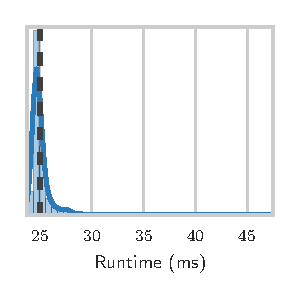
\includegraphics[width=\textwidth]{img/runtimes_histogram_1}
% \vspace{-1.5em} % Shrink vertical padding
% \caption{}
% \label{fig:runtimes-histogram-1}
% \end{subfigure}
% ~%
% \begin{subfigure}[h]{.32\columnwidth}
% \centering
% 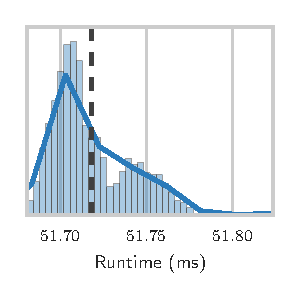
\includegraphics[width=\textwidth]{img/runtimes_histogram_2}
% \vspace{-1.5em} % Shrink vertical padding
% \caption{}
% \label{fig:runtimes-histogram-2}
% \end{subfigure}
% ~%
% \begin{subfigure}[h]{.32\columnwidth}
% \centering
% 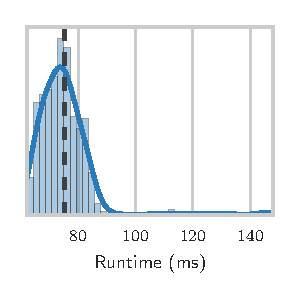
\includegraphics[width=\textwidth]{img/runtimes_histogram_3}
% \vspace{-1.5em} % Shrink vertical padding
% \caption{}
% \label{fig:runtimes-histogram-3}
% \end{subfigure}
% \\
% \begin{subfigure}[h]{.32\columnwidth}
% \centering
% 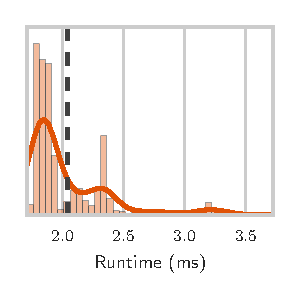
\includegraphics[width=\textwidth]{img/runtimes_histogram_4}
% \vspace{-1.5em} % Shrink vertical padding
% \caption{}
% \label{fig:runtimes-histogram-4}
% \end{subfigure}
% ~%
% \begin{subfigure}[h]{.32\columnwidth}
% \centering
% 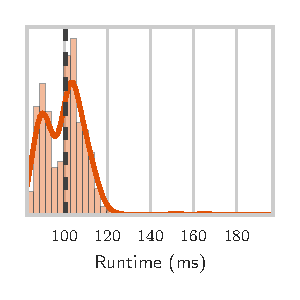
\includegraphics[width=\textwidth]{img/runtimes_histogram_5}
% \vspace{-1.5em} % Shrink vertical padding
% \caption{}
% \label{fig:runtimes-histogram-5}
% \end{subfigure}
% ~%
% \begin{subfigure}[h]{.32\columnwidth}
% \centering
% 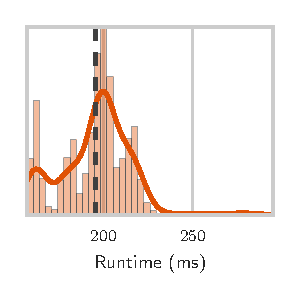
\includegraphics[width=\textwidth]{img/runtimes_histogram_6}
% \vspace{-1.5em} % Shrink vertical padding
% \caption{}
% \label{fig:runtimes-histogram-6}
% \end{subfigure}
% \\
% \begin{subfigure}[h]{.32\columnwidth}
% \centering
% 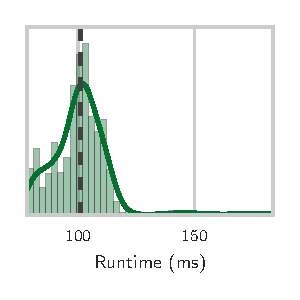
\includegraphics[width=\textwidth]{img/runtimes_histogram_7}
% \vspace{-1.5em} % Shrink vertical padding
% \caption{}
% \label{fig:runtimes-histogram-7}
% \end{subfigure}
% ~%
% \begin{subfigure}[h]{.32\columnwidth}
% \centering
% 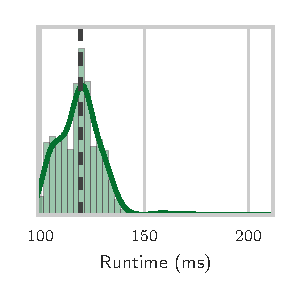
\includegraphics[width=\textwidth]{img/runtimes_histogram_8}
% \vspace{-1.5em} % Shrink vertical padding
% \caption{}
% \label{fig:runtimes-histogram-8}
% \end{subfigure}
% ~%
% \begin{subfigure}[h]{.32\columnwidth}
% \centering
% 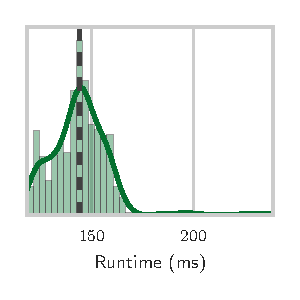
\includegraphics[width=\textwidth]{img/runtimes_histogram_9}
% \vspace{-1.5em} % Shrink vertical padding
% \caption{}
% \label{fig:runtimes-histogram-9}
% \end{subfigure}
% \caption[Distribution of stencil code runtimes]{%
%   Distribution of runtime samples for test cases from three
%   devices. Each plot contains a 35-bin histogram of 1000 samples, and
%   a fitted kernel density estimate with bandwidth 0.3. The sample mean
%   is shown as a vertical dashed line. The top row are from the Intel
%   i5-4570, the second row from the Nvidia GTX 590, and the third row
%   from the AMD Tahiti 7970. In some of the plots, the distribution of
%   runtimes is bimodal, and skewed to the lower end of the runtimes
%   range.%
% }
% \label{fig:runtime-histograms}
% \end{figure}


\begin{figure}
  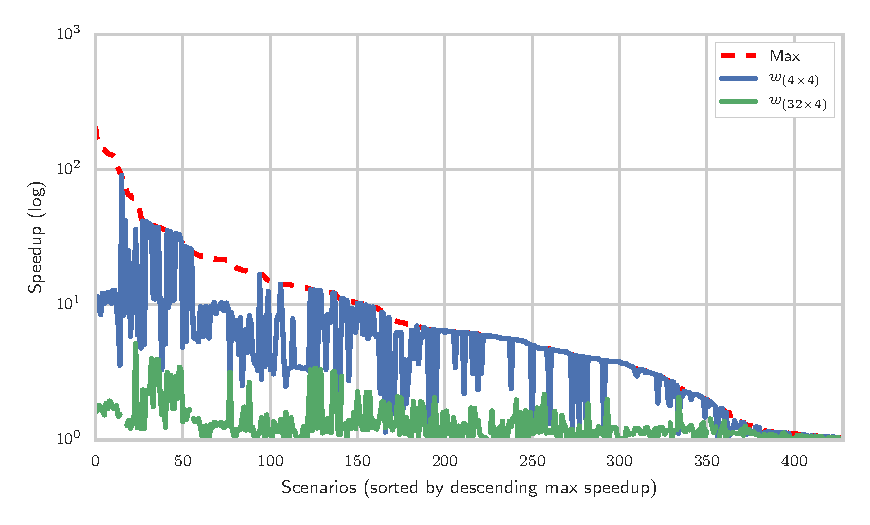
\includegraphics[width=\columnwidth]{img/max_speedups}
  \caption[Workgroup size speedups]{%
    Speedup of oracle workgroup size over: the worst performing
    workgroup size for each scenario (\emph{Max}), the statically
    chosen workgroup size that provides the best overall performance
    ($w_{(4 \times 4)}$), and the human expert selected parameter
    ($w_{(32 \times 4)}$). Note that the human expert parameter is not
    legal for all scenarios.%
  }
\label{fig:speedups}
\end{figure}

For a given scenario $s$, the ratio of the workgroups sizes from
$W_{legal}(s)$ which provide the longest and shortest mean runtimes is
used to calculate an upper bound for the possible performance
influence of workgroup size:
%
\begin{equation}
r_{max}(s) = r(s, \argmax_{w \in W_{legal}(s)} t(s,w), \Omega(s))
\end{equation}
%
When applied to each scenario $s \in S$ of the experimental results,
we find the average of speedup upper bounds to be $15.14\times$ (min
$1.03\times$, max $207.72\times$). This demonstrates the importance of
tuning stencil workgroup sizes --- if chosen incorrectly, the runtime
of stencil programs can be extended by up to $207.72\times$. Note too
that for 5 of the scenarios, the speedup of the best over worst
workgroup sizes is $\le 5\%$.
% TODO: t-test for this!
For these scenarios, there is little benefit to autotuning; however,
this represents only 1.1\% of the tested scenarios. For 50\% of the
scenarios, the speedup of the best over worst workgroup sizes is
$\ge 6.19\times$.


% The complex interaction between processes competing for the finite
% resources of a system introduces many sources for noise in program
% runtime measurements. Before making any judgements about the relative
% performance of optimisation configurations, we must establish the
% level of noise present in these measurements. To do this, we evaluate
% the distribution of runtimes for a randomly selected 1000 test cases,
% recording 1000 runtime observations for each. We can then produce
% fine-grained histograms of runtimes for individual test
% cases.

Figure~\ref{fig:runtime-histograms} shows the distributions of 1000
runtimes for each of nine test cases, from three devices. The plots
show that the distribution of runtimes is not always Gaussian; rather,
it is sometimes bimodal, and generally skewed to the lower end of the
runtime range, with a long ``tail'' to the right. This fits our
intuition that programs have a hard \emph{minimum} runtime enforced by
the time taken to execute the instructions of a program, and that
noise introduced to the system extends this runtime. For example,
preempting an OpenCL process on a CPU so that another process may run
may cause the very long tail visible in
Figure~\ref{fig:runtimes-histogram-1}.

As the number of samples increases, we
should expect the size of the confidence interval to shrink. This is
illustrated in Figure~\ref{fig:ci-trends}, which plots the average
size of 95\% confidence intervals across the 1000 test cases,
normalised to their respective means, as a function of sample
size. It shows the diminishing returns that increasing sample size
provides. For example, increasing the sample count from 10 to 30
results in an approximate 50\% reduction in confidence interval
size. Increasing the sample size from 30 to 50 results in only a
25\% reduction.

\begin{figure}
\centering
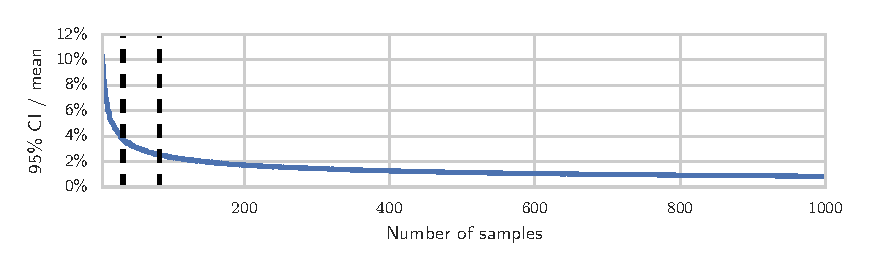
\includegraphics[width=\columnwidth]{img/ci_trend}
\caption[Confidence interval size vs.\ sample count]{%
  Ratio of confidence interval to mean as a function of sample
  count. Two dashed lines indicate the confidence intervals at the
  minimum (3.7\%) and mean (2.5\%) number of samples used in the
  experimental dataset.%
}
\label{fig:ci-trends}
\end{figure}

By comparing the average confidence interval at different sample
counts against the full experiment results of 269813 test cases, we
can assert with 95\% confidence that the true mean for each test case
is within 2.5\% of the sample mean (given the average number of
samples per test case), or 3.7\% in the worst case (at the minimum
number of samples). Since the differences between baseline and optimal
workgroup sizes is often well in excess of 100\%, there is no overlap
of confidence intervals between competing workgroup sizes.


\begin{figure}
\centering
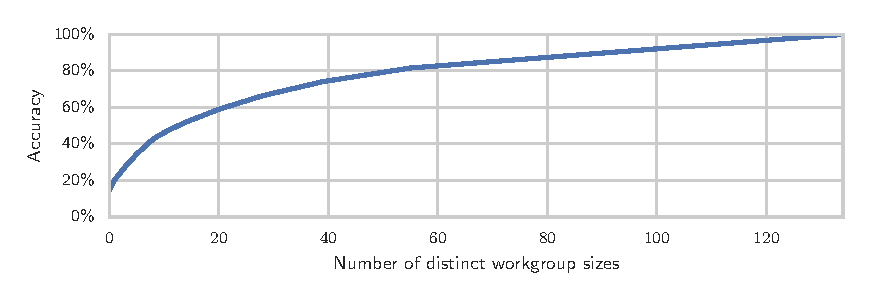
\includegraphics[width=\columnwidth]{img/num_params_oracle.pdf}
\caption[Oracle accuracy vs.\ number of workgroup sizes]{%
  Accuracy compared to the oracle as a function of the number of
  workgroup sizes used. The best accuracy that can be achieved using a
  single statically chosen workgroup size is 15\%. Achieving 50\%
  oracle accuracy requires a minimum of 14 distinct workgroup sizes.%
}
\label{fig:oracle-accuracy}
\end{figure}

For each scenario $s$, the oracle workgroup size $\Omega(s)$ is the
workgroup size which resulted in the lowest mean runtime. If the
performance of stencils were independent of workgroup size, we would
expect that the oracle workgroup size would remain constant across all
scenarios $s \in S$. Instead, we find that there are 135 unique oracle
workgroup sizes, with 31.5\% of scenarios having a unique workgroup
size. This demonstrates the difficult in attempting to tune for
\emph{optimal} parameter values, since 14 distinct workgroup sizes are
needed to achieve just 50\% of the oracle accuracy
(Figure~\ref{fig:oracle-accuracy}), although it is important to make
the distinction that oracle \emph{accuracy} and \emph{performance} are
not equivalent.

In the original implementation of the SkelCL stencil
skeleton~\cite{Breuer2013}, \citeauthor{Breuer2013} selected a
workgroup size of $w_{(32 \times 4)}$ in an evaluation of 4 stencil
operations on a Tesla S1070 system. We can use this as an additional
parameter to compare the relative performance of workgroup sizes
against. However, the $w_{(32 \times 4)}$ workgroup size is invalid
for 2.6\% of scenarios, as it is refused in 11 test cases. By device,
those are: 3 on the GTX 690, 6 on the i5-2430M, and 2 on the i5-4570.
For the scenarios where $w_{(32 \times 4)}$ \emph{is} legal, the human
expert chosen workgroup size achieves an impressive geometric mean of
79.2\% of the oracle performance. The average speedup of oracle
workgroup sizes over the workgroup size selected by a human expert is
$1.37\times$ (min $1.0\times$, max $5.17\times$). Since the workgroup
size selected by the human expert is not legal for all scenarios, we
will examine the effectiveness of heuristics for tuning workgroup
size.

% % \subsubsection{Heuristics}

In this subsection we will consider the effectiveness of instead
selecting workgroup size using two types of heuristics. The first,
using the maximum workgroup size returned by the OpenCL device and
kernel APIs to select the workgroup size adaptively. The second, using
per-device heuristics, in which the workgroup size is selected based
on the specific architecture that a stencil is operating on.

% \paragraph{Using maximum legal size}

A common approach taken by OpenCL developers is to set the workgroup
size for a kernel based on the maximum legal workgroup size queried
from the OpenCL APIs. For example, to set the size of 2D workgroup, a
developer the square root of the (scalar) maximum wgsize to set the
number of columns and rows (since $w_c \cdot w_r$ must be
$< W_{\max}(s)$). To consider the effectiveness of this approach, we
group the workgroup size performances based on the ratio of the
maximum allowed for each scenario. We can also perform this for each
of the two dimensions --- rows and columns --- of the stencil
workgroup size.

Figure~\ref{fig:performance-wgsizes} shows the distribution of
runtimes when grouped this way, demonstrating that the performance of
(legal) workgroup sizes are not correlated with the maximum workgroup
sizes $W_{\max}(s)$. However, when considering individual components,
we observe that the best median workgroup size performances are
achieved with a number of columns that is between 10\% and 20\% of the
maximum, and a number of rows that is between 0\% and 10\% of the
maximum.

% \paragraph{Per-device workgroup sizes}

\begin{table}
  \scriptsize
  \centering
  \begin{tabular}{lllp{.9cm}p{.9cm}}
    \toprule
    Device &         Oracle & Legality & Perf.\ min & Perf.\ avg. \\
    \midrule
    AMD Tahiti 7970 &   $48\times 4$ &      1.0 &       0.54 &        0.91 \\
    Intel i5-2430M &  $64\times 16$ &      0.8 &       0.37 &        0.91 \\
    Intel i5-4570 &   $88\times 8$ &     0.89 &       0.33 &        0.89 \\
    Intel i7-3820 &  $40\times 24$ &     0.95 &       0.76 &        0.97 \\
    NVIDIA GTX 590 &  $12\times 2$ &      0.8 &        0.2 &         0.9 \\
    NVIDIA GTX 690 &   $64\times 4$ &     0.93 &       0.32 &        0.84 \\
    NVIDIA GTX TITAN &   $64\times 4$ &      1.0 &       0.26 &        0.81 \\
    \textbf{CPUs} &   $88\times 8$ &     0.88 &       0.33 &        0.91 \\
    \textbf{GPUs} &   $64\times 4$ &     0.76 &       0.26 &        0.86 \\
    \bottomrule
  \end{tabular}
  \caption[Performance of tuning with a per-device heuristic]{%
    Selecting workgroup size using a per-device heuristic. The mode
    optimal workgroup size for each device type is evaluated
    based on legality, and relative performance to the oracle (minimum
    and average) when legal.%
  }
  \label{tab:heuristic-dev}
\end{table}

One possible technique to selecting workgroup size is to tune
particular values for each targeted execution device. This approach is
sometimes adopted for cases with particularly high requirements for
performance on a single platform, so it produces an interesting
contrast to evaluating a machine learning approach, which attempts to
predict workgroup sizes for unseen platforms without the need for an
expensive exploration phase on the new platform.

Figure~\ref{fig:performances} shows the performance of workgroup sizes
relative to the oracle across scenarios grouped by: kernel, device,
and dataset. When grouped like this, a number of observations can
made. First is that not all of the kernels are sensitive to tuning
workgroup size to the same degree. The \emph{sobel} kernel has the
lowest median performance, indicating that it is the most profitable
to tune, while the \emph{threshold} kernel is the least
profitable. Similarly, the Intel i7-3820 is far less amenable to
tuning than the other devices, while the Intel i5-4570 is the most
sensitive to the workgroup size parameter. Such variances in the
distributions of workgroup sizes suggest that properties underlying
the architecture, kernel, and dataset all contribute towards the
proper selection of workgroup size.

To test the performance of a per-device heuristic for selecting
workgroup size, we group the scenarios by device, and compare the
relative performance of all workgroup sizes for each group of
scenarios. The most frequently optimal workgroup size $\bar{w}$ for
each device is selected, and the legality and performance of each
scenario using that workgroup size is evaluated.
Table~\ref{tab:heuristic-dev} shows the results of this evaluation.
The GTX 690 and GTX TITAN share the same $\bar{w}_{(64 \times 4)}$
value, while every other device has a unique optimum. The general case
performance of these per-device parameters is very good, although
legality is only assured for the GTX TITAN and AMD 7970 (which did not
refuse any parameters). However, the worst case performance of
per-device workgroup sizes is poor for all except the i7-3820 (which
is least sensitive to tuning), suggesting that device alone is not
capable of reliably informing the choice of workgroup size.


\begin{figure}
  \begin{subfigure}[h]{\columnwidth}
    \centering
    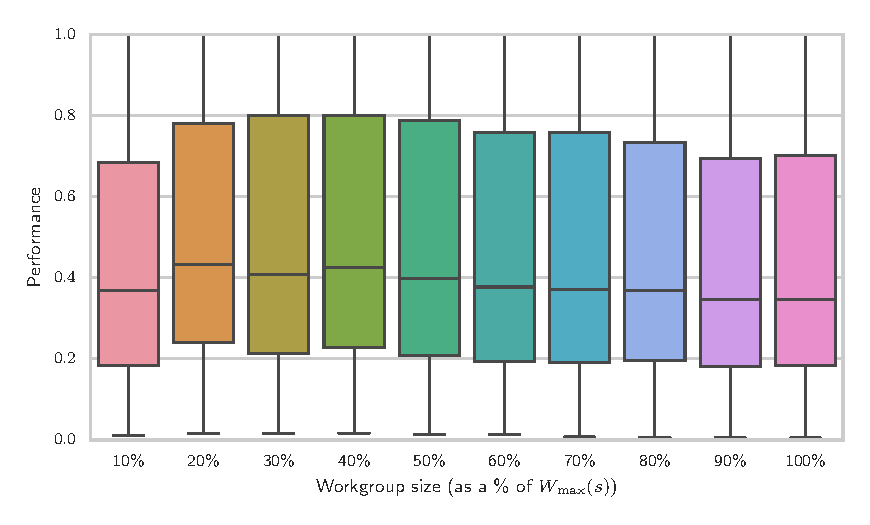
\includegraphics[width=\columnwidth]{img/performance_max_wgsize}
    \vspace{-1.5em} % Shrink vertical padding
    \caption{}
    \label{fig:performance-max-wgsize}
  \end{subfigure}
  \\
  \begin{subfigure}[h]{.48\columnwidth}
    \centering
    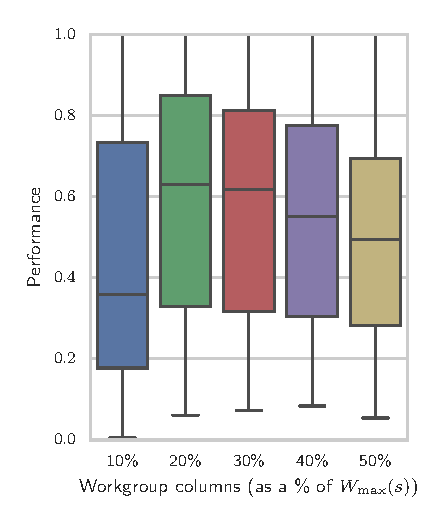
\includegraphics[width=\columnwidth]{img/performance_max_c}
    \vspace{-1.5em} % Shrink vertical padding
    \caption{}
    \label{fig:performance-wg-c}
  \end{subfigure}
  ~%
  \begin{subfigure}[h]{.48\columnwidth}
    \centering
    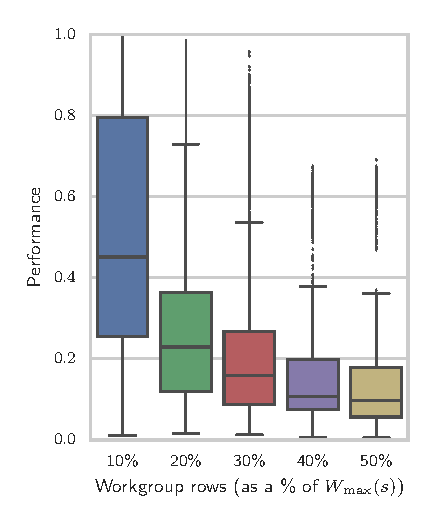
\includegraphics[width=\columnwidth]{img/performance_max_r}
    \vspace{-1.5em} % Shrink vertical padding
    \caption{}
    \label{fig:performance-wg-r}
  \end{subfigure}

  \caption[Workgroup size performances vs.\ size]{%
    Comparing workgroup performance relative to the oracle as function
    of: (\subref{fig:performance-max-wgsize})~maximum legal size,
    (\subref{fig:performance-wg-c})~number of columns, and
    (\subref{fig:performance-wg-r})~ number of rows. Each workgroup
    size is normalised to the maximum allowed for that scenario, $W_{\max}(s)$.%
  }
  \label{fig:performance-wgsizes}
\end{figure}

\begin{figure}
  \begin{subfigure}[h]{\columnwidth}
    \centering
    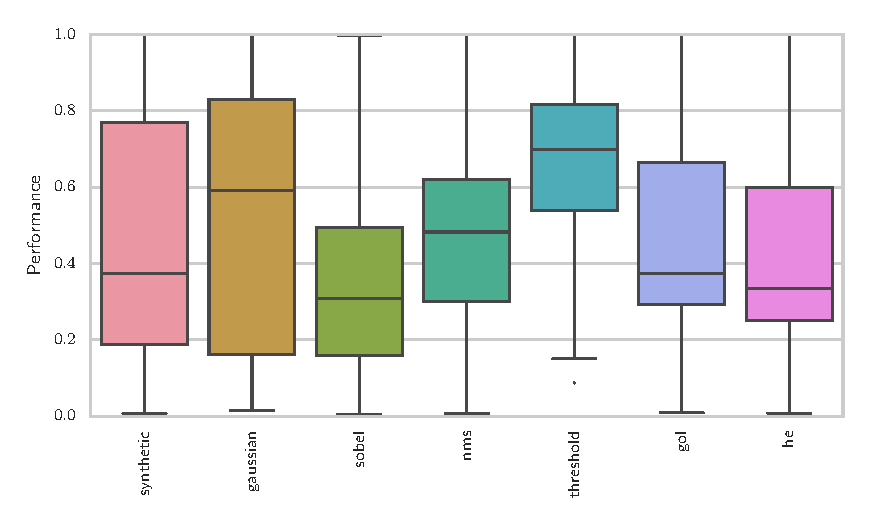
\includegraphics[width=\columnwidth]{img/performance_kernels.pdf}
    \vspace{-1.5em} % Shrink vertical padding
    \caption{}
    \label{fig:performance-kernels}
  \end{subfigure}
  \\
  \begin{subfigure}[h]{.48\columnwidth}
    \centering
    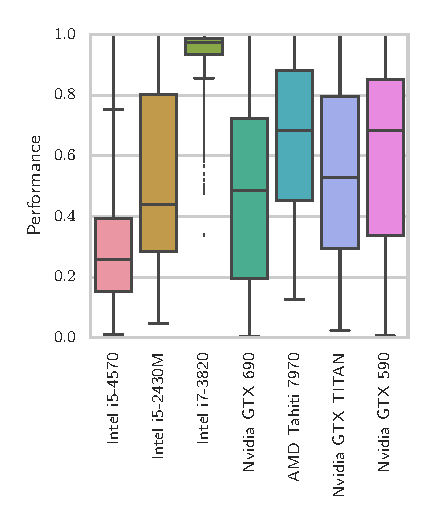
\includegraphics[width=\columnwidth]{img/performance_devices.pdf}
    \vspace{-1.5em} % Shrink vertical padding
    \caption{}
    \label{fig:performance-devices}
  \end{subfigure}
  ~%
  \begin{subfigure}[h]{.48\columnwidth}
    \centering
    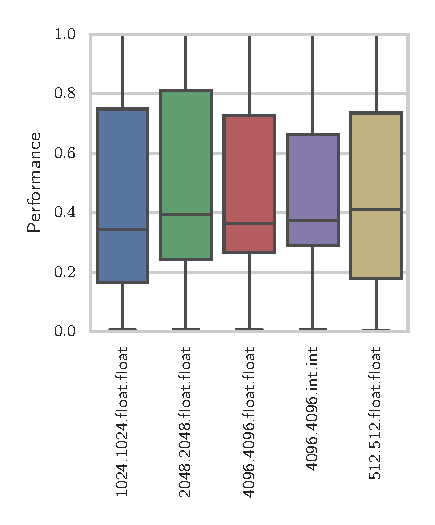
\includegraphics[width=\columnwidth]{img/performance_datasets.pdf}
    \vspace{-1.5em} % Shrink vertical padding
    \caption{}
    \label{fig:performance-datasets}
  \end{subfigure}
  \caption[Workgroup size performances across device, kernel, and dataset]{%
    Performance relative to the oracle of workgroup sizes across all
    test cases, grouped by: (\subref{fig:performance-kernels})~kernels,
    (\subref{fig:performance-devices})~devices, and
    (\subref{fig:performance-datasets})~datasets.%
  }
  \label{fig:performances}
\end{figure}


% % \subsubsection{Summary}

% In this subsection we have explored the performance impact of the
% workgroup size optimisation space. By comparing the relative
% performance of an average of 629 workgroup sizes for each of 429
% scenarios, the following conclusions can be drawn:

% \begin{enumerate}
% \item The performance of a workgroup size for a particular scenario
%   depends properties of the hardware, software, and dataset.
% \item The performance gap between the best and workgroup sizes for a
%   particular combination of hardware, software, and dataset is up to
%   $207.72\times$.
% \item Not all workgroup sizes are legal, and the space of legal
%   workgroup sizes cannot statically be determined. Adaptive tuning of
%   workgroup size is required to ensure reliable performance.
% \item Differing scenarios have wildly different optimal workgroup
%   sizes, and the best performance can be achieved using static tuning
%   is optimal for only 15\% of scenarios.
% \end{enumerate}
% %
% % I believe this presents a compelling case for the development of an
% % autotuner which can select the optimal workgroup size at runtime.
% %
% In the following subsection, we will evaluate the performance of OmniTune
% for selecting workgroup sizes.



% With the exception of the ZeroR, which predicts \emph{only} the
% baseline workgroup size $w_{\left( 4 \times 4 \right)}$, the
% classifiers achieve good speedups over the baseline. Average
% classification speedups across all validation sets range between
% $4.61\times$ and $5.05\times$. Figures~\ref{fig:class-syn}
% and~\ref{fig:class-arch} show a summary of results using 10-fold
% cross-validation and cross-device validation, respectively.  The
% highest average speedup is achieved by SMO, and the lowest by Naive
% Bayes. The difference between average speedups is not significant
% between the types of classifier, with the exception of SimpleLogistic,
% which performs poorly when trained with synthetic benchmarks and
% tested against real-world programs. This suggests the model
% over-fitting to features of the synthetic benchmarks which are not
% shared by the real-world
% tests.

% By isolating the test cases where classifiers predicted an illegal or
% refused parameter, we can directly compare the relative effectiveness
% of each fallback handler. The fallback handler with the best average
% case performance is \textsc{NearestNeighbour}, with an average speedup
% across all classifiers and validation sets of $5.26\times$. The
% speedup of \textsc{Random} fallback handler is $3.69\times$, and
% $1.0\times$ for \textsc{Baseline}. Figure~\ref{fig:fallback-speedups}
% plots the speedups of each fallback handler for all of these isolated
% test cases. Interestingly, both the lowest and highest speedups are
% achieved by the \textsc{Random} fallback handler, since it essentially
% performs a random exploration of the optimisation space. However, the
% \textsc{NearestNeighbour} fallback handler provides consistently
% greater speedups for the majority of test cases, indicating that it
% successfully exploits the structure of the optimisation spaces.

% Figures~\ref{fig:runtime-class-xval} and ~\ref{fig:speedup-class-xval}
% show a summary of results for classification using regressors to
% predict program runtimes and speedups, respectively. Of the two
% regression techniques, predicting the \emph{speedup} of workgroup
% sizes is much more successful than predicting the \emph{runtime}. This
% is most likely caused by the inherent difficulty in predicting the
% runtime of arbitrary programs, where dynamic factors such as flow
% control and loop bounds are not captured by the kernel features used
% in OmniTune, which instead use simple static static instruction counts
% and densities. The average speedup achieved by predicting runtimes is
% $4.14\times$. For predicting speedups, the average is $5.57\times$.
% Tables~\ref{tab:class}, \ref{tab:runtime-class},
% and~\ref{tab:speedup-class} show mean performances and speedups for:
% J48 classifier using the \textsc{NearestNeighour} fallback strategy,
% classification using runtime regression, and classification using
% speedup regression, respectively.

% If we eliminate the 2.6\% of test cases for which the workgroup size
% of $w_{(32 \times 4)}$ is illegal, we can compare the performance of
% OmniTune directly against the human expert chosen workgroup
% size. Figure~\ref{fig:speedup-distributions} compares the speedups of
% all such validation instances over the human expert parameter, for
% each autotuning technique. The speedup distributions show consistent
% classification results for the five classification techniques, with
% the speedup at the lower quartile for all classifiers being
% $\ge 1.0\times$. The IQR for all classifiers is $< 0.5$, but there are
% outliers with speedups both well below $1.0\times$ and well above
% $2.0\times$. In contrast, the speedups achieved using runtime
% regression have a lower range, but also a lower median and a larger
% IQR. Clearly, runtime regression is the least effective of the
% evaluated autotuning techniques. Speedup regression is more
% successful, with the highest median speedup of all the
% techniques. However, it also has a large IQR and the lower quartile
% has a speedup value well below 1, meaning that for more than 25\% of
% test instances, the workgroup size selected did not perform as well as
% the human expert selected workgroup size.

% % The lower average speedup attained by speedup regression over the
% % J48 classifier belies the fact that the \emph{median} speedup is
% % much greater, at $1.33 \times$.


% \begin{table}
% \scriptsize
% \centering
% \begin{tabular}{llll}
% \toprule
%               Job &    Performance &            Speedup &       Human Expert \\
% \midrule
%           10-fold &           68\% &       $4.13\times$ &       $0.88\times$ \\
%         Synthetic &           78\% &       $3.81\times$ &       $1.06\times$ \\
%            Device &           69\% &       $3.89\times$ &       $0.97\times$ \\
%            Kernel &           74\% &       $4.36\times$ &       $1.04\times$ \\
%           Dataset &           72\% &       $4.33\times$ &       $0.98\times$ \\
%  \textbf{Average} &  \textbf{70\%} &  $\bm{4.14\times}$ &  $\bm{0.92\times}$ \\
% \bottomrule
% \end{tabular}
% \caption{Validation results for runtime regression.}
% \label{tab:runtime-class}
% \end{table}
% \begin{table}
% \scriptsize
% \centering
% \begin{tabular}{llll}
% \toprule
%               Job &    Performance &            Speedup &       Human Expert \\
% \midrule
%           10-fold &           89\% &       $5.67\times$ &       $1.10\times$ \\
%         Synthetic &           86\% &       $4.48\times$ &       $1.19\times$ \\
%            Device &           85\% &       $5.18\times$ &       $1.15\times$ \\
%            Kernel &           88\% &       $5.38\times$ &       $1.15\times$ \\
%           Dataset &           88\% &       $5.53\times$ &       $1.13\times$ \\
%  \textbf{Average} &  \textbf{89\%} &  $\bm{5.57\times}$ &  $\bm{1.12\times}$ \\
% \bottomrule
% \end{tabular}
% \caption{Validation results for speedup regression.}
% \label{tab:speedup-class}
% \end{table}



The prediction costs using regression are significantly greater than
using classifiers. This is because, while a classifier makes a single
prediction, the number of predictions required of a regressor grows
with the size of $W_{\max}(s)$, since classification with regression
requires making predictions for all
$w \in \left\{ w | w < W_{\max}(s) \right\}$. The fastest classifier
is J48, due to the it's simplicity (it can be implemented as a
sequence of nested \texttt{if}/\texttt{else} statements).

% From an evaluation of 17 different autotuning techniques using 5
% different types of validation sets, the following conclusions about
% autotuning performance can be drawn:
% %
% \begin{itemize}
% \item In the case of classifiers predicting illegal workgroup sizes,
%   the best fallback strategy is to select the closest legal workgroup
%   size.
% \item The performance of predicted workgroup sizes for unseen devices
%   is within 8\% of the performance for known devices.
% \item Predicting the \emph{runtime} of stencils is the least effective
%   of the evaluated autotuning techniques, achieving an average of only
%   68\% of the available performance.
% \item Predicting the \emph{speedup} of workgroup sizes provides the
%   highest median speedup, but more frequently predicts a poorly
%   performing workgroup size then the classifiers.
% \item Classification using regression costs an order of magnitude more
%   time than using classifiers. The J48 classifier has the lowest
%   overhead.
% \end{itemize}

In the original implementation of the SkelCL stencil
skeleton~\cite{Breuer2013}, \citeauthor{Breuer2013} selected a
workgroup size of $w_{(32 \times 4)}$ in an evaluation of 4 stencil
operations on a Tesla S1070 system. We can use this as an additional
parameter to compare the relative performance of workgroup sizes
against. However, the $w_{(32 \times 4)}$ workgroup size is invalid
for 2.6\% of scenarios, as it is refused in 11 test cases. By device,
those are: 3 on the GTX 690, 6 on the i5-2430M, and 2 on the i5-4570.
For the scenarios where $w_{(32 \times 4)}$ \emph{is} legal, the human
expert chosen workgroup size achieves an impressive geometric mean of
79.2\% of the oracle performance. The average speedup of oracle
workgroup sizes over the workgroup size selected by a human expert is
$1.37\times$ (min $1.0\times$, max $5.17\times$). Since the workgroup
size selected by the human expert is not legal for all scenarios, we
will examine the effectiveness of heuristics for tuning workgroup
size.


\subsection{Autotuning overheads}


\subsection{Collective Tuning}

\begin{table}
\scriptsize
\centering
\begin{tabular}{llll}
\toprule
              Job &    Performance &            Speedup &       Human Expert \\
\midrule
\textbf{10-fold} & \textbf{92\%} & \textbf{$5.65\times$} & \textbf{$1.26\times$} \\
        Synthetic &           92\% &       $4.79\times$ &       $1.13\times$ \\
           Device &           85\% &       $5.23\times$ &       $1.17\times$ \\
           Kernel &           89\% &       $5.43\times$ &       $1.21\times$ \\
          Dataset &           91\% &       $5.63\times$ &       $1.25\times$ \\
 % \textbf{Average} &  \textbf{90\%} &  $\bm{5.45\times}$ &  $\bm{1.22\times}$ \\
\bottomrule
\end{tabular}
\caption{Validation results for J48 and \textsc{NearestNeighbour}
  classification.}
\label{tab:class}
\end{table}


\subsection{Classifier selection}

\begin{figure}
\centering
\begin{subfigure}[t]{0.48\columnwidth}
\centering
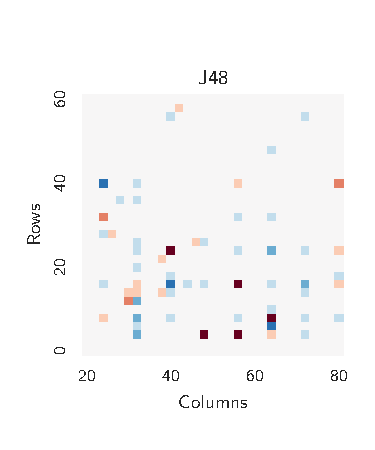
\includegraphics[width=\columnwidth]{img/heatmap_1}
\vspace{-1.5em} % Shrink vertical padding
\caption{}
\label{fig:class-hmaps-1}
\end{subfigure}
\begin{subfigure}[t]{0.48\columnwidth}
\centering
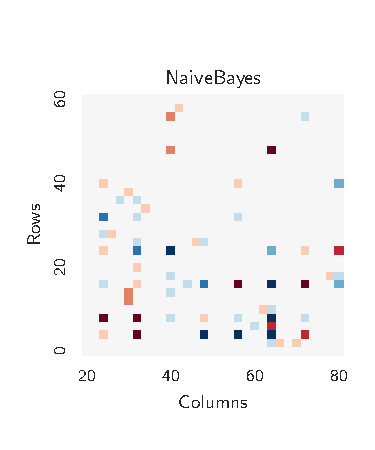
\includegraphics[width=\columnwidth]{img/heatmap_2}
\vspace{-1.5em} % Shrink vertical padding
\caption{}
\label{fig:class-hmaps-2}
\end{subfigure}
\\
\begin{subfigure}[t]{0.48\columnwidth}
\centering
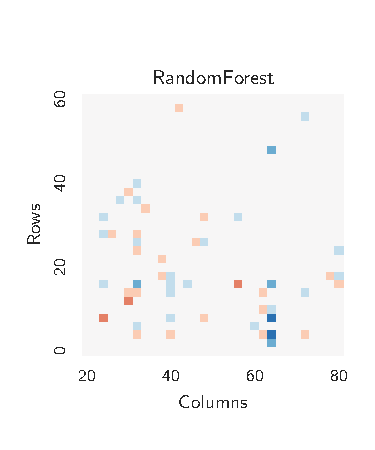
\includegraphics[width=\columnwidth]{img/heatmap_3}
\vspace{-1.5em} % Shrink vertical padding
\caption{}
\label{fig:class-hmaps-3}
\end{subfigure}
\begin{subfigure}[t]{0.48\columnwidth}
\centering
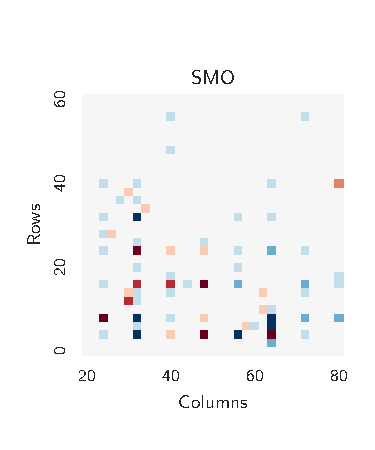
\includegraphics[width=\columnwidth]{img/heatmap_5}
\vspace{-1.5em} % Shrink vertical padding
\caption{}
\label{fig:class-hmaps-4}
\end{subfigure}
\caption{%
  Heatmaps of classification errors for a subset of the optimisation
  space using four different classifiers. The shading in each cells
  indicates if it is predicted less frequently (blue), ore more
  frequently (red) than it is optimal. Colour gradients are normalised
  across plots.%
}
\label{fig:class-hmaps}
\end{figure}



\section{Related Work}\label{sec:related}


% \subsubsection{Training with Synthetic Benchmarks}

% The use of synthetic benchmarks for providing empirical performance
% evaluations dates back to as early as 1974~\cite{Curnow1976}. The
% \emph{automatic generation} of such synthetic benchmarks is a more
% recent innovation, serving the purpose initially of stress-testing
% increasingly complex software systems for behaviour validation and
% automatic bug detection~\cite{Verplaetse2000,Godefroid2008}. A range
% of techniques have been developed for these purposes, ranging from
% applying random mutations to a known dataset to generate test stimuli,
% to so-called ``whitebox fuzz testing'' which analyses program traces
% to explore the space of a program's control flow. Csmith is one such
% tool which generates randomised C source programs for the purpose of
% automatically detecting compiler bugs~\cite{Yang2012}.

% A method for the automatic generation of synthetic benchmarks for the
% purpose of \emph{performance} tuning is presented
% in~\cite{Chiu2015}. \citeauthor{Chiu2015} use template substitution
% over a user-defined range of values to generate training programs with
% a statistically controlled range of features. A Perl preprocessor
% generates output source codes from an input description using a custom
% input language Genesis. Genesis is more flexible than the system
% presented in this thesis, supporting substitution of arbitrary
% sources. The authors describe an application of their tool for
% generating OpenCL stencil kernels, but do not report any performance
% results.


% \subsection{Performance Tuning for Heterogeneous Parallelism}

% As briefly discussed in Subsection~\ref{subsec:gpgpu}, the complex
% interactions between optimisations and heterogeneous hardware makes
% performance tuning for heterogeneous parallelism a difficult
% task. Performant GPGPU programs require careful attention from the
% developer to properly manage data layout in DRAM, caching, diverging
% control flow, and thread communication. The performance of programs
% depends heavily on fully utilising zero-overhead thread scheduling,
% memory bandwidth, and thread grouping. \citeauthor{Ryoo2008a}
% illustrate the importance of these factors by demonstrating speedups
% of up to $432\times$ for matrix multiplication in CUDA by appropriate
% use of tiling and loop unrolling~\cite{Ryoo2008a}. The importance of
% proper exploitation of local shared memory and synchronisation costs
% is explored in~\cite{Lee2010}.

% In~\cite{Chen2014}, data locality optimisations are automated using a
% description of the hardware and a memory-placement-agnostic
% compiler. The authors demonstrate impressive speedups of up to
% $2.08\times$, although at the cost of requiring accurate memory
% hierarchy descriptor files for all targeted hardware. The descriptor
% files must be hand generated, requiring expert knowledge of the
% underlying hardware in order to properly exploit memory locality.

% Data locality for nested parallel patterns is explored in~\cite{Lee}.
% The authors use an automatic mapping strategy for nested parallel
% skeletons on GPUs, which uses a custom intermediate representation and
% a CUDA code generator, achieving $1.24\times$ speedup over hand
% optimised code on 7 of 8 Rodinia benchmarks.

% Reduction of the GPGPU optimisation space is demonstrated
% in~\cite{Ryoo2008}, using the common subset of optimal configurations
% across a set of training examples. This technique reduces the search
% space by 98\%, although it does not guarantee that for a new program,
% the reduced search space will include the optimal configuration.

% \citeauthor{Magni2014} demonstrated that thread coarsening of OpenCL
% kernels can lead to speedups in program performance between
% $1.11\times$ and $1.33\times$ in~\cite{Magni2014}. The authors achieve
% this using a machine learning model to predict optimal thread
% coarsening factors based on the static features of kernels, and an
% LLVM function pass to perform the required code transformations.

% A framework for the automatic generation of OpenCL kernels from
% high-level programming concepts is described in~\cite{Steuwer2015}. A
% set of rewrite rules is used to transform high-level expressions to
% OpenCL code, creating a space of possible implementations. This
% approach is ideologically similar to that of PetaBricks, in that
% optimisations are made through algorithmic choice, although in this
% case the transformations are performed automatically at the compiler
% level. The authors report performance on a par with that of hand
% written OpenCL kernels.


% \subsection{Autotuning Algorithmic Skeletons}

An enumeration of the optimisation space of Intel Thread Building
Blocks in~\cite{Contreras2008} shows that runtime knowledge of the
available parallel hardware can have a significant impact on program
performance. \citeauthor{Collins2012} exploit this
in~\cite{Collins2012}, first using Principle Components Analysis to
reduce the dimensionality of the space of possible optimisation
parameters, followed by a search of parameter values to optimise
program performance by a factor of $1.6\times$ over values chosen by a
human expert. In~\cite{Collins2013}, they extend this using static
feature extraction and nearest neighbour classification to further
prune the search space, achieving an average 89\% of the oracle
performance after evaluating 45 parameters.

\citeauthor{Dastgeer2011} developed a machine learning based autotuner
for the SkePU skeleton library in~\cite{Dastgeer2011}. Training data
is used to predict the optimal execution device (i.e.\ CPU, GPU) for a
given program by predicting execution time and memory copy overhead
based on problem size. The autotuner only supports vector operations,
and there is limited cross-architecture
evaluation. In~\cite{Dastgeer2015a}, the authors extend SkePU to
improve the data consistency and transfer overhead of container types,
reporting up to a $33.4\times$ speedup over the previous
implementation.


% \subsection{Code Generation and Autotuning for Stencils}

% Stencil codes have a variety of computationally expensive uses from
% fluid dynamics to quantum mechanics. Efficient, tuned stencil kernels
% are highly sought after, with early work in \citeyear{Bolz2003} by
% \citeauthor{Bolz2003} demonstrating the capability of GPUs for
% massively parallel stencil operations~\cite{Bolz2003}. In the
% resulting years, stencil codes have received much attention from the
% performance tuning research community.

% \citeauthor{Ganapathi2009} demonstrated early attempts at autotuning
% multicore stencil codes in~\cite{Ganapathi2009}, drawing upon the
% successes of statistical machine learning techniques in the compiler
% community, as discussed in
% Subsection~\ref{subsec:iterative-compilation}. They present an autotuner
% which can achieve performance up to 18\% better than that of a human
% expert. From a space of 10 million configurations, they evaluate the
% performance of a randomly selected 1500 combinations, using Kernel
% Canonical Correlation Analysis to build correlations between tunable
% parameter values and measured performance targets. Performance targets
% are L1 cache misses, TLB misses, cycles per thread, and power
% consumption. The use of KCAA restricts the scalability of their system
% as the complexity of model building grows exponentially with the
% number of features. In their evaluation, the system requires two hours
% of compute time to build the KCAA model for only 400 seconds of
% benchmark data. They present a compelling argument for the use of
% energy efficiency as an optimisation target in addition to runtime,
% citing that it was the power wall that lead to the multicore
% revolution in the first place. Their choice of only 2 benchmarks and 2
% platforms makes the evaluation of their autotuner somewhat limited.

% \citeauthor{Berkeley2009} targeted 3D stencils code performance
% in~\cite{Berkeley2009}. Stencils are decomposed into core blocks,
% sufficiently small to avoid last level cache capacity misses. These
% are then further decomposed to thread blocks, designed to exploit
% common locality threads may have within a shared cache or local
% memory. Thread blocks are divided into register blocks in order to
% take advantage of data level parallelism provided by the available
% registers. Data allocation is optimised on NUMA systems. The
% performance evaluation considers speedups of various optimisations
% with and without consideration for host/device transfer overhead.

% \citeauthor{Kamil2010} present an autotuning framework
% in~\cite{Kamil2010} which accepts as input a Fortran 95 stencil
% expression and generates tuned shared-memory parallel implementations
% in Fortan, C, or CUDA. The system uses an IR to explore autotuning
% transformations, enumerating a subset of the optimisation space and
% recording only a single execution time for each configuration,
% reporting the fastest. They demonstrate their system on 4
% architectures using 3 benchmarks, with speedups of up to $22\times$
% compared to serial implementations. The CUDA code generator does not
% optimise for the GPU memory hierarchy, using only global memory. As
% demonstrated in this thesis, improper utilisation of local memory can
% hinder program performance by two orders of magnitude. There is no
% directed search or cross-program learning.

% In~\cite{Zhang2013a}, \citeauthor{Zhang2013a} present a code generator
% and autotuner for 3D Jacobi stencil codes. Using a DSL to express
% kernel functions, the code generator performs substitution from one of
% two CUDA templates to create programs for execution on GPUs. GPU
% programs are parameterised and tuned for block size, block dimensions,
% and whether input data is stored in read only texture memory. This
% creates an optimisation space of up to 200 configurations. In an
% evaluation of 4 benchmarks, the authors report impressive performance
% that is comparable with previous implementations of iterative Jacobi
% stencils on GPUs~\cite{Holewinski2012, Phillips2010}. The dominating
% parameter is shown to be block dimensions, followed by block size,
% then read only memory. The DSL presented in the paper is limited to
% expressing only Jacobi Stencils applications. Critically, their
% autotuner requires a full enumeration of the parameter space for each
% program. Since there is no indication of the compute time required to
% gather this data, it gives the impression that the system would be
% impractical for the needs of general purpose stencil computing. The
% autotuner presented in this thesis overcomes this drawback by learning
% parameter values which transfer to unseen stencils, without the need
% for an expensive tuning phase for each program and architecture.
% % TODO: Depending on results of cross-architecture validation, this
% % last claim may not hold up.
% %
% % The majority of applications tested are memory bound. Does this
% % transfer to computer bound?

% In~\cite{Christen2011}, \citeauthor{Christen2011} presentf a DSL for
% expressing stencil codes, a C code generator, and an autotuner for
% exploring the optimisation space of blocking and vectorisation
% strategies. The DSL supports stencil operations on arbitrarily
% high-dimensional grids. The autotuner performs either an exhaustive,
% multi-run Powell search, Nelder Mead, or evolutionary search to find
% optimal parameter values. They evaluate their system on two CPUS and
% one GPU using 6 benchmarks. A comparison of tuning results between
% different GPU architectures would have been welcome, as the results
% presented in this thesis show that devices have different responses to
% optimisation parameters. The authors do not present a ratio of the
% available performance that their system achieves, or how the
% performance of optimisations vary across benchmarks or devices.

% A stencil grid can be decomposed into smaller subsections so that
% multiple GPUs can operate on each subsection independently. This
% requires a small overlapping region where each subsection meets ---
% the halo region --- to be shared between devices. For iterative
% stencils, values in the halo region must be synchronised between
% devices after each iteration, leading to costly communication
% overheads. One possible optimisation is to deliberately increase the
% size of the halo region, allowing each device to compute updated
% values for the halo region, instead of requiring a synchronisation of
% shared state. This reduces the communication costs between GPUs, at
% the expense of introducing redundant computation. Tuning the size of
% this halo region is the goal of PARTANS~\cite{Lutz2013}, an autotuning
% framework for multi-GPU stencil computations. \citeauthor{Lutz2013}
% explore the effect of varying the size of the halo regions using six
% benchmark applications, finding that the optimal halo size depends on
% the size of the grid, the number of partitions, and the connection
% mechanism (i.e.\ PCI express). The authors present an autotuner which
% determines problem decomposition and swapping strategy offline, and
% performs an online search for the optimal halo size. The selection of
% overlapping halo region size compliments the selection of workgroup
% size which is the subject of this thesis. However, PARTANS uses a
% custom DSL rather than the generic interface provided by SkelCL, and
% PARTANS does not learn the results of tuning across programs, or
% across multiple runs of the same program.


% \subsection{Summary}

There is already a wealth of research literature on the topic
autotuning which begs the question, why isn't the majority of software
autotuned? In this section I attempted to answer the question by
reviewing the state of the art in the autotuning literature, with
specific reference to auotuning for GPUs and stencil codes. The bulk
of this research falls prey of one of two shortcomings. Either they
identify and develop a methodology for tuning a particular
optimisation space but then fail to develop a system which can
properly exploit this (for example, by using machine learning to
predict optimal values across programs), or they present an autotuner
which targets too specific of a class of optimisations to be widely
applicable. This project attempts to address both of those
shortcomings by expending great effort to deliver a working
implementation which users can download and use without any setup
costs, and by providing a modular and extensible framework which
allows rapid targeting of new autotuning platforms, enabled by a
shared autotuning logic and distributed training data. The following
section outlines the design of this system.


\paragraph{OpenTuner} Similar in both name and intent is OpenTuner, a
\ldots


\paragraph{Collective Mind} In~\cite{Saclay2010,Memon2013,Fursin2014},
\citeauthor{Fursin2014} advocate a collaborative and ``big data''
driven approach to autotuning, arguing that the challenges facing the
widespread adoption of autotuning and machine learning methodologies
can be attributed to: a lack of common, diverse benchmarks and
datasets; a lack of common experimental methodology; problems with
continuously changing hardware and software stacks; and the difficulty
to validate techniques due to a lack of sharing in publications. They
propose a system for addressing these concerns, the Collective Mind
knowledge system, which, while in early stages of ongoing development,
is intended to provide a modular infrastructure for sharing autotuning
performance data and related artifacts across the internet. In
addition to sharing performance data, the approach taken in this work
emphasises the collective \emph{exploitation} of such performance
data, so that data gathered from one device may be used to inform the
autotuning decisions of another. This requires each device to maintain
local caches of shared data to remove the network overhead that would
be present from querying a single centralised data store during
execution of a hot path. The current implementation of Collective Mind
uses a NoSQL JSON format for storing performance data. The relational
schema used in this thesis offers greater scaling performance and
lower storage overhead as the amount of performance data grows.


\section{Conclusions}\label{sec:conclusions}

As the trend towards higher core counts and increasing parallelism
continues, the need for high level, accessible abstractions to manage
such parallelism will continue to go. Autotuning proves a valuable aid
for achieving these goals, providing the benefits of low level
performance tuning while maintaining ease of use, without burdening
developers with optimisation concerns. As the need for autotuned
parallelism rises, the desire for collaborative techniques for sharing
performance data must be met with systems capable of supporting this
cross-platform learning.

In this work, we have presented an attempt to provide such a system,
by designing a novel framework which has the benefits of fast,
``always-on'' autotuning, while being able to synchronise data with
global repositories of knowledge which others may contribute to. The
framework provides an interface for autotuning which is sufficiently
generic to be easily re-purposed to target a range of optimisation
parameters.

To demonstrate the utility of this framework, we implemented a
frontend for predicting the workgroup size of OpenCL kernels for
SkelCL stencil codes. The publicly available implementation
\footnote{\url{https://github.com/ChrisCummins/omnitune}} predicts
workgroup sizes for OpenCL stencil skeleton kernels in order to
minimise their runtime on CPUs and multi-GPU systems. This
optimisation space is complex, non linear, and critical for the
performance of stencil kernels, with up to a $207.72\times$ slowdown
if an improper value is picked. Selecting the correct workgroup size
is difficult --- requiring a knowledge of the kernel, dataset, and
underlying architecture. The challenge is increased even more so by
inconsistencies in the underlying system which cause some workgroup
sizes to fail completely. Of the 269813 combinations of workgroup
size, device, program, and dataset tested; only a \emph{single}
workgroup size was valid for all test cases, and achieved only 24\% of
the available performance. The value selected by human experts was
invalid for 2.6\% of test cases. Autotuning in this space requires a
system which is resilient these challenges, and several techniques
were implemented to address them.

Runtime performance of autotuned stencil kernels is very promising,
achieving an average 90\% of the available performance with only a 3ms
autotuning overhead. Even ignoring the cases for which the human
expert selected workgroup size is invalid, this provides a
$1.33\times$ speedup, or a $5.57\times$ speedup over the best
performance that can be achieved using static tuning. Classification
performance is comparable when predicting workgroup sizes for both
unseen programs and unseen devices. I believe that the combination of
performance improvements and the collaborative nature of OmniTune
makes for a compelling case for the use of autotuning as a key
component for enabling performant, high level parallel programming.

The cost of offline training with OmniTune could be reduced by
exploring the use of adaptive sampling plans, such as presented
in~\cite{Leather2009}. This could reduce the number of runtime samples
required to distinguish good from bad optimisation parameter values.

Collaborative training --- hive mind for selecting training
parameters, and built-in redundancy checking/validation

TODO: deltas for push and pull, scalability for huge datasets

TODO: involuntary training requests, or non-binary selectors between
training and performance

%
% \appendix
% \section{Appendix Title}
%
% This is the text of the appendix, if you need one.
%

\acks

This work was supported by the UK Engineering and Physical Sciences
Research Council under grants EP/L01503X/1 for the University of
Edinburgh School of Informatics Centre for Doctoral Training in
Pervasive Parallelism
(\url{http://pervasiveparallelism.inf.ed.ac.uk/}),\\* EP/H044752/1
(ALEA), and EP/M015793/1 (DIVIDEND).

% We recommend abbrvnat bibliography style.

\label{bibliography}
\printbibliography


\end{document}
